\documentclass[a4paper]{article}

\def\npart{III}

\def\ntitle{Analytic Number Theory}
\def\nlecturer{T.\ F.\ Bloom}

\def\nterm{Lent}
\def\nyear{2019}

\ifx \nauthor\undefined
  \def\nauthor{Qiangru Kuang}
\else
\fi

\ifx \ntitle\undefined
  \def\ntitle{Template}
\else
\fi

\ifx \nauthoremail\undefined
  \def\nauthoremail{qk206@cam.ac.uk}
\else
\fi

\ifx \ndate\undefined
  \def\ndate{\today}
\else
\fi

\title{\ntitle}
\author{\nauthor}
\date{\ndate}

%\usepackage{microtype}
\usepackage{mathtools}
\usepackage{amsthm}
\usepackage{stmaryrd}%symbols used so far: \mapsfrom
\usepackage{empheq}
\usepackage{amssymb}
\let\mathbbalt\mathbb
\let\pitchforkold\pitchfork
\usepackage{unicode-math}
\let\mathbb\mathbbalt%reset to original \mathbb
\let\pitchfork\pitchforkold

\usepackage{imakeidx}
\makeindex[intoc]

%to address the problem that Latin modern doesn't have unicode support for setminus
%https://tex.stackexchange.com/a/55205/26707
\AtBeginDocument{\renewcommand*{\setminus}{\mathbin{\backslash}}}
\AtBeginDocument{\renewcommand*{\models}{\vDash}}%for \vDash is same size as \vdash but orginal \models is larger
\AtBeginDocument{\let\Re\relax}
\AtBeginDocument{\let\Im\relax}
\AtBeginDocument{\DeclareMathOperator{\Re}{Re}}
\AtBeginDocument{\DeclareMathOperator{\Im}{Im}}
\AtBeginDocument{\let\div\relax}
\AtBeginDocument{\DeclareMathOperator{\div}{div}}

\usepackage{tikz}
\usetikzlibrary{automata,positioning}
\usepackage{pgfplots}
%some preset styles
\pgfplotsset{compat=1.15}
\pgfplotsset{centre/.append style={axis x line=middle, axis y line=middle, xlabel={$x$}, ylabel={$y$}, axis equal}}
\usepackage{tikz-cd}
\usepackage{graphicx}
\usepackage{newunicodechar}

\usepackage{fancyhdr}

\fancypagestyle{mypagestyle}{
    \fancyhf{}
    \lhead{\emph{\nouppercase{\leftmark}}}
    \rhead{}
    \cfoot{\thepage}
}
\pagestyle{mypagestyle}

\usepackage{titlesec}
\newcommand{\sectionbreak}{\clearpage} % clear page after each section
\usepackage[perpage]{footmisc}
\usepackage{blindtext}

%\reallywidehat
%https://tex.stackexchange.com/a/101136/26707
\usepackage{scalerel,stackengine}
\stackMath
\newcommand\reallywidehat[1]{%
\savestack{\tmpbox}{\stretchto{%
  \scaleto{%
    \scalerel*[\widthof{\ensuremath{#1}}]{\kern-.6pt\bigwedge\kern-.6pt}%
    {\rule[-\textheight/2]{1ex}{\textheight}}%WIDTH-LIMITED BIG WEDGE
  }{\textheight}% 
}{0.5ex}}%
\stackon[1pt]{#1}{\tmpbox}%
}

%\usepackage{braket}
\usepackage{thmtools}%restate theorem
\usepackage{hyperref}

% https://en.wikibooks.org/wiki/LaTeX/Hyperlinks
\hypersetup{
    %bookmarks=true,
    unicode=true,
    pdftitle={\ntitle},
    pdfauthor={\nauthor},
    pdfsubject={Mathematics},
    pdfcreator={\nauthor},
    pdfproducer={\nauthor},
    pdfkeywords={math maths \ntitle},
    colorlinks=true,
    linkcolor={red!50!black},
    citecolor={blue!50!black},
    urlcolor={blue!80!black}
}

\usepackage{cleveref}



% TODO: mdframed often gives bad breaks that cause empty lines. Would like to switch to tcolorbox.
% The current workaround is to set innerbottommargin=0pt.

%\usepackage[theorems]{tcolorbox}





\usepackage[framemethod=tikz]{mdframed}
\mdfdefinestyle{leftbar}{
  %nobreak=true, %dirty hack
  linewidth=1.5pt,
  linecolor=gray,
  hidealllines=true,
  leftline=true,
  leftmargin=0pt,
  innerleftmargin=5pt,
  innerrightmargin=10pt,
  innertopmargin=-5pt,
  % innerbottommargin=5pt, % original
  innerbottommargin=0pt, % temporary hack 
}
%\newmdtheoremenv[style=leftbar]{theorem}{Theorem}[section]
%\newmdtheoremenv[style=leftbar]{proposition}[theorem]{proposition}
%\newmdtheoremenv[style=leftbar]{lemma}[theorem]{Lemma}
%\newmdtheoremenv[style=leftbar]{corollary}[theorem]{corollary}

\newtheorem{theorem}{Theorem}[section]
\newtheorem{proposition}[theorem]{Proposition}
\newtheorem{lemma}[theorem]{Lemma}
\newtheorem{corollary}[theorem]{Corollary}
\newtheorem{axiom}[theorem]{Axiom}
\newtheorem*{axiom*}{Axiom}

\surroundwithmdframed[style=leftbar]{theorem}
\surroundwithmdframed[style=leftbar]{proposition}
\surroundwithmdframed[style=leftbar]{lemma}
\surroundwithmdframed[style=leftbar]{corollary}
\surroundwithmdframed[style=leftbar]{axiom}
\surroundwithmdframed[style=leftbar]{axiom*}

\theoremstyle{definition}

\newtheorem*{definition}{Definition}
\surroundwithmdframed[style=leftbar]{definition}

\newtheorem*{slogan}{Slogan}
\newtheorem*{eg}{Example}
\newtheorem*{ex}{Exercise}
\newtheorem*{remark}{Remark}
\newtheorem*{notation}{Notation}
\newtheorem*{convention}{Convention}
\newtheorem*{assumption}{Assumption}
\newtheorem*{question}{Question}
\newtheorem*{answer}{Answer}
\newtheorem*{note}{Note}
\newtheorem*{application}{Application}

%operator macros

%basic
\DeclareMathOperator{\lcm}{lcm}

%matrix
\DeclareMathOperator{\tr}{tr}
\DeclareMathOperator{\Tr}{Tr}
\DeclareMathOperator{\adj}{adj}

%algebra
\DeclareMathOperator{\Hom}{Hom}
\DeclareMathOperator{\End}{End}
\DeclareMathOperator{\id}{id}
\DeclareMathOperator{\im}{im}
\DeclarePairedDelimiter{\generation}{\langle}{\rangle}

%groups
\DeclareMathOperator{\sym}{Sym}
\DeclareMathOperator{\sgn}{sgn}
\DeclareMathOperator{\inn}{Inn}
\DeclareMathOperator{\aut}{Aut}
\DeclareMathOperator{\GL}{GL}
\DeclareMathOperator{\SL}{SL}
\DeclareMathOperator{\PGL}{PGL}
\DeclareMathOperator{\PSL}{PSL}
\DeclareMathOperator{\SU}{SU}
\DeclareMathOperator{\UU}{U}
\DeclareMathOperator{\SO}{SO}
\DeclareMathOperator{\OO}{O}
\DeclareMathOperator{\PSU}{PSU}

%hyperbolic
\DeclareMathOperator{\sech}{sech}

%field, galois heory
\DeclareMathOperator{\ch}{ch}
\DeclareMathOperator{\gal}{Gal}
\DeclareMathOperator{\emb}{Emb}



%ceiling and floor
%https://tex.stackexchange.com/a/118217/26707
\DeclarePairedDelimiter\ceil{\lceil}{\rceil}
\DeclarePairedDelimiter\floor{\lfloor}{\rfloor}


\DeclarePairedDelimiter{\innerproduct}{\langle}{\rangle}

%\DeclarePairedDelimiterX{\norm}[1]{\lVert}{\rVert}{#1}
\DeclarePairedDelimiter{\norm}{\lVert}{\rVert}



%Dirac notation
%TODO: rewrite for variable number of arguments
\DeclarePairedDelimiterX{\braket}[2]{\langle}{\rangle}{#1 \delimsize\vert #2}
\DeclarePairedDelimiterX{\braketthree}[3]{\langle}{\rangle}{#1 \delimsize\vert #2 \delimsize\vert #3}

\DeclarePairedDelimiter{\bra}{\langle}{\rvert}
\DeclarePairedDelimiter{\ket}{\lvert}{\rangle}




%macros

%general

%divide, not divide
\newcommand*{\divides}{\mid}
\newcommand*{\ndivides}{\nmid}
%vector, i.e. mathbf
%https://tex.stackexchange.com/a/45746/26707
\newcommand*{\V}[1]{{\ensuremath{\symbf{#1}}}}
%closure
\newcommand*{\cl}[1]{\overline{#1}}
%conjugate
\newcommand*{\conj}[1]{\overline{#1}}
%set complement
\newcommand*{\stcomp}[1]{\overline{#1}}
\newcommand*{\compose}{\circ}
\newcommand*{\nto}{\nrightarrow}
\newcommand*{\p}{\partial}
%embed
\newcommand*{\embed}{\hookrightarrow}
%surjection
\newcommand*{\surj}{\twoheadrightarrow}
%power set
\newcommand*{\powerset}{\mathcal{P}}

%matrix
\newcommand*{\matrixring}{\mathcal{M}}

%groups
\newcommand*{\normal}{\trianglelefteq}
%rings
\newcommand*{\ideal}{\trianglelefteq}

%fields
\renewcommand*{\C}{{\mathbb{C}}}
\newcommand*{\R}{{\mathbb{R}}}
\newcommand*{\Q}{{\mathbb{Q}}}
\newcommand*{\Z}{{\mathbb{Z}}}
\newcommand*{\N}{{\mathbb{N}}}
\newcommand*{\F}{{\mathbb{F}}}
%not really but I think this belongs here
\newcommand*{\A}{{\mathbb{A}}}

%asymptotic
\newcommand*{\bigO}{O}
\newcommand*{\smallo}{o}

%probability
\newcommand*{\prob}{\mathbb{P}}
\newcommand*{\E}{\mathbb{E}}

%vector calculus
\newcommand*{\gradient}{\V \nabla}
\newcommand*{\divergence}{\gradient \cdot}
\newcommand*{\curl}{\gradient \cdot}

%logic
\newcommand*{\yields}{\vdash}
\newcommand*{\nyields}{\nvdash}

%differential geometry
\renewcommand*{\H}{\mathbb{H}}
\newcommand*{\transversal}{\pitchfork}
\renewcommand{\d}{\mathrm{d}} % exterior derivative

%number theory
\newcommand*{\legendre}[2]{\genfrac{(}{)}{}{}{#1}{#2}}%Legendre symbol


\usepackage{cancel}

\newtheorem*{fact}{Fact}
\theoremstyle{definition}
\newtheorem*{conjecture}{Conjecture}

\begin{document}

\begin{titlepage}
  \begin{center}
    
\includegraphics[width=0.6\textwidth]{logo.jpg}\par
    \vspace{1cm}
    {\scshape\huge Mathematics Tripos \par}
    \vspace{2cm}
    {\huge Part \npart \par}
    \vspace{0.6cm}
    {\Huge \bfseries \ntitle \par}
    \vspace{1.2cm}
    {\Large\nterm, \nyear \par}
    \vspace{2cm}
    
    {\large \emph{Lectures by } \par}
    \vspace{0.2cm}
    {\Large \scshape \nlecturer}
    
    \vspace{0.5cm}
    {\large \emph{Notes by }\par}
    \vspace{0.2cm}
    {\Large \scshape \href{mailto:\nauthoremail}{\nauthor}}
 \end{center}
\end{titlepage}

\tableofcontents

\setcounter{section}{-1}

\section{Introduction}

Analytic number theory is the study of numbers using analysis. In particular it answers quantitative questions. ``Numbers'' means natural numbers in this course, which excludes \(0\).

\begin{eg}\leavevmode
  \begin{enumerate}
  \item How many primes are there? We know there are infinitely many but can we have a more precise answer? Let \(\pi(x)\) be the number of primes smaller than or equal to \(x\). Then by the famous prime number theorem, \(\pi(x) \sim \frac{x}{\log x}\).
  \item How may twin primes are there? It is not known whethere there are infinitely many. From 2014 Zhang, Maynard, Polymath, there are infinitely many primes at most \(246\) apart. It's been conjectured that the asymptotic bound is \(\sim \frac{x}{(\log x)^2}\).
  \item How many primes are there congruent to \(a\) mod \(q\) where \((a, q) = 1\)? There are infinitely many by Dirichlet's theorem. The guess is \(\frac{1}{\varphi(q)}\frac{x}{\log x}\). This is known for small \(q\).
  \end{enumerate}
\end{eg}

The course is divided into four parts:
\begin{enumerate}
\item elementary techniques (using real analysis),
\item sieve methods,
\item Riemann zeta function/Prime number theorem (using complex analysis),
\item primes in arithmetic progression.
\end{enumerate}

\section{Elementary techniques}

Review of asymptotic notations:
\begin{itemize}
\item Landau notation: \(f(x) = O(g(x))\) if there is \(C > 0\) such that \(|f(x)| \leq C|g(x)|\) for all large enough \(x\).
\item Vinogradov notation: \(f \ll g\) is the same as \(f = O(g)\).
\item \(f \sim g\) if \(\lim_{x \to \infty} \frac{f(x)}{g(x)} = 1\), i.e.\ \(f = (1 + o(1)) g\).
\item \(f = o(g)\) if \(\lim_{x \to \infty} \frac{f(x)}{g(x)} = 0\).
\end{itemize}

\subsection{Arithmetic functions}

These are just functions \(f: \N \to \C\). An important operation for multiplicative number theory is \emph{multiplicative convolution}\index{multiplicative convolution}
\[
  f * g(n) = \sum_{ab = n} f(a)g(b)
\]

\begin{eg}\leavevmode
  \begin{enumerate}
  \item \(1(n) = 1\) for all \(n\). Caution: this is not identity on \(\N\).
  \item \emph{Möbius function}\index{Möbius function}
    \[
      \mu(n) =
      \begin{cases}
        (-1)^k & \text{ if } n = p_1 \dots p_k \\
        0 & \text{ if \(n\) is divisible by a square}
      \end{cases}
    \]
  \item \emph{Liouville function}
    \[
      \lambda(n) = (-1)^k
    \]
    if \(n = p_1 \dots p_k\) where \(p_i\)'s are not necessarily distinct.
  \item \emph{divisor function}
    \[
      \tau(n) = \#d \text{ such that } d \divides n = \sum_{ab = n} 1 = 1 * 1(n).
    \]
    This is sometimes also denoted by \(d(n)\).
  \end{enumerate}
\end{eg}

\begin{definition}[multiplicative function]\index{multiplicative function}
  An arithmetic function \(f\) is \emph{multiplicative} if
  \[
    f(nm) = f(n)f(m)
  \]
  whenever \((n, m) = 1\).
\end{definition}

In particular a multiplicative function is determined by its values on prime powers \(f(p^k)\).

\begin{fact}
  If \(f\) and \(g\) are multiplicative then so is \(f * g\).
\end{fact}

\begin{eg}
  \(1, \mu, \lambda, \tau\) are multiplicative. \(\log n\) is not multiplicative.
\end{eg}

\begin{fact}[Möbius inversion]\index{Möbius inversion}
  \(1 * f = g\) if and only if \(\mu * g = f\). That is,
  \[
    \sum_{d \divides n} f(d) = g(n)
  \]
  if and only if
  \[
    \sum_{d \divides n} g(d) \mu(\frac{n}{d}) = f(n).
  \]

  For example
  \[
    \sum_{d \divides n} \mu(d) =
    \begin{cases}
      1 & n = 1 \\
      0 & \text{otherwise}
    \end{cases}
    = 1 * \mu (n)
  \]
  is multiplicative so enough to check the identity for prime powers. If \(n = p^k\) then \(\{d: d \divides n\} = \{1, p, \dots, p^k\}\) so LHS equals to \(1 - 1 + 0 + \dots = 0\) unless \(k = 1\) when LHS equals to \(\mu(1) = 1\).
\end{fact}

Our goal is to study primes. Our first might be that we shall work with
\[
  1_p(n) =
  \begin{cases}
    1 & n \text{ prime} \\
    0 & \text{otherwise}
  \end{cases}
\]
as then \(\pi(x) = \sum_{1 \leq n \leq x} 1_p(n)\). But this is very awkward to work with, as to begin with, this is not multiplicative. Instead, we are going to work almost exclusively with \emph{von Mangoldt function}\index{von Mangoldt function}
\[
  \Lambda(n) =
  \begin{cases}
    \log p & n = p^k \\
    0 & \text{otherwise}
  \end{cases}
\]
``assign weight \(\log p\) to prime power \(n\)''

\begin{lemma}
  \[
    1 * \Lambda = \log.
  \]
  and
  \[
    \mu * \log = \Lambda.
  \]
\end{lemma}

\begin{proof}
  The second part follows from Möbius inversion. Thus if \(n = p_1^{k_1} \dots p_r^{k_r}\),
  \begin{align*}
    1 * \Lambda(n)
    &= \sum_{d \divides n} \Lambda(d)
    = \sum_{i = 1}^r \sum_{j = 1}^{k_i} \Lambda(p_i^j) \\
    &= \sum_{i = 1}^r \sum_{j = 1}^{k_i} \log(p_i)
    = \sum_{i = 1}^r k_i \log p_i \\
    &= \sum_{i = 1}^r \log (p_i^{k_i})
    = \log n
  \end{align*}
\end{proof}

Therefore
\begin{align*}
  \Lambda(n)
  &= \sum_{d \divides n} \mu(d) \log(\frac{n}{d}) \\
  &= \log n \sum_{d \divides n} \mu(d) - \sum_{d \divides n} \mu(d) \log d \\
  &= - \sum_{d \divides n} \mu(d) \log d
\end{align*}
For example
\[
  \sum_{1 \leq n \leq x} \Lambda(n)
  = - \sum_{1 \leq n \leq x} \sum_{d \divides n} \mu(d) \log d
  = - \sum_{d \leq x} \mu(d) \log d \left(\sum_{1 \leq n \leq x, d \divides n} 1\right)
\]
by reversing summation. But now the term in the inner summation is very easy to understand:
\[
  \sum_{1 \leq n \leq x, d \divides n} 1 = \floor*{\frac{x}{d}} = \frac{x}{d} + O(1).
\]
Thus
\[
  \sum_{1 \leq n \leq x} \Lambda(n)
  = -x \sum_{d \leq x} \mu(d) \frac{\log d}{d} + O\left(\sum_{d \leq x} \mu(d) \log d\right).
\]
We'll see more of these examples.

\subsection{Summation}

Given an arithmetic function \(f\), we can ask for estimates of \(\sum_{1 \leq n \leq x} f(n)\). We say that \(f\) has \emph{average order}\index{average order} \(g\) if
\[
  \sum_{1 \leq n \leq x} f(n) \sim x g(x).
\]
``average size of \(f\) is \(g\)''.

\begin{eg}\leavevmode
  \begin{enumerate}
  \item \(f = 1\) then
    \[
      \sum_{1 \leq n \leq x} f(x) = \floor{x} = x + O(1) \sim x
    \]
    so average order of \(1\) is \(1\).
  \item \(f(n) = n\):
    \[
      \sum_{1 \leq n \leq x} n \sim \frac{x^2}{2}
    \]
    so average of \(n\) is \(\frac{n}{2}\).
  \end{enumerate}
\end{eg}

\begin{lemma}[partial summation]\index{partial summation}
  If \((a_n)\) is a sequence of complex numbers and \(f\) is such that \(f'\) is continuous. Then
  \[
    \sum_{1 \leq n \leq x} a_n f(n) = A(x) f(x) - \int_1^x A(t)f'(t) dt
  \]
  where \(A(x) = \sum_{1 \leq n \leq x} a_n\).
\end{lemma}

This is the discrete analogus of integration by parts.

\begin{proof}
  Suppose \(x = N\) is an integer. Note that \(a_n = A(n) - A(n - 1)\), so
  \begin{align*}
    \sum_{1 \leq n \leq N} a_nf(n)
    &= \sum_{1 \leq n \leq N} f(n) (A(n) - A(n - 1)) \\
    &= A(N)f(N) - \sum_{n = 1}^{N - 1} A(n) (f(n + 1) - f(n))
  \end{align*}
  Now
  \[
    f(n + 1) - f(n) = \int_n^{n + 1} f'(t) dt
  \]
  so
  \begin{align*}
    \sum_{1 \leq n \leq N} a_n f(n)
    &= A(N)f(N) - \sum_{n = 1}^{N - 1} A(n) \int_n^{n + 1} f'(t) dt \\
    &= A(N)f(N) - \int_1^N A(t) f'(t) dt
  \end{align*}
  where the last step is because \(A(n) = A(t)\) for \(t \in [n, n + 1)\).

  If \(N = \floor x\) then
  \[
    A(x)f(x)
    = A(N)f(x)
    = A(N) f(N) + \int_N^x f'(t) dt.
  \]
\end{proof}

As a simple application

\begin{lemma}
  \[
    \sum_{1 \leq n \leq x} \frac{1}{n} = \log x + \gamma + O(\frac{1}{x}).
  \]
\end{lemma}

\begin{proof}
  Partial summation with \(f(x) = \frac{1}{x}\) and \(a_n = 1\), so \(A(x) = \floor x\). Therefore
  \begin{align*}
    \sum_{1 \leq n \leq x} \frac{1}{n}
    &= \frac{\floor x}{x} + \int_1^x \frac{\floor t}{t^2} dt
    \intertext{Write \(\floor t= t - \{t\}\),} \\
    &= 1 + O(\frac{1}{x}) + \int_1^x \frac{1}{t} dt - \int_1^x \frac{\{t\}}{t^2} dt \\
    &= 1 + O(\frac{1}{x}) + \log x - \int_1^\infty \frac{\{t\}}{t^2} dt + \underbrace{\int_x^\infty \frac{\{t\}}{t^2} dt}_{\leq \int_x^\infty \frac{1}{t^2} dt \leq \frac{1}{x}} \\
    &= \gamma + O(\frac {1}{x}) + \log x + O(\frac{1}{x}) \\
    &= \log x + \gamma + O(\frac{1}{x})
  \end{align*}
\end{proof}

This is an amazing result and the only thing we did is to replace the discrete summation by the continuous analogue to it. In essence this is the whole reason analytic number theory works.

\(\gamma\) can be seen as a measure of the difference between between \(\log\) and its discrete approximation. It is called \emph{Euler-Mascheroni constant}\index{Euler-Mascheroni constant}.
Surprisingly little is known about \(\gamma\). It is approximately \(0.577\dots\). We don't even know if \(\gamma\) is rational or not.

\begin{lemma}
  \[
    \sum_{1 \leq n \leq x} \log n = x \log x - x + O(\log x).
  \]
\end{lemma}

\begin{proof}
  Partial summation with \(f(x) = \log x, a_n = 1\) so \(A(x) = \floor{x}\). As a side note, in the previous example, most error comes from the integral term (the mass is evenly distributed). By constrast in this example most error comes from the ``sum'' term.
  \begin{align*}
    \sum_{1 \leq n \leq x} \log n
    &= \floor{x} \log x - \int_1^x \frac{\floor{t}}{t} dt \\
    &= x \log x + O(\log x) - \int_1^x dt + O(\int_1^x \frac{1}{t}dt) \\
    &= x \log x + O(\log x) - x + O(\log x)
  \end{align*}
\end{proof}

\subsection{Divisor function}

Recall that
\[
  \tau(n) = 1 * 1(n) = \sum_{ab = n} 1 = \sum_{d \divides n} 1.
\]

\begin{theorem}
  \[
    \sum_{1 \leq n \leq x} \tau(n) = x \log x + (2 \gamma - 1) x + O(x^{1/2})
  \]
  so in particular average order of \(\tau\) is \(\log\).
\end{theorem}

\begin{proof}
  First attempt:
  \begin{align*}
    \sum_{1 \leq n \leq x} \tau(n)
    &= \sum_{1 \leq n \leq x} \sum_{d \divides n} 1
    = \sum_{1 \leq d \leq x} \sum_{1 \leq n \leq x, d \divides n} 1 \\
    &= \sum_{1 \leq d \leq x} \floor*{\frac{x}{d}} \\
    &= \sum_{1 \leq d \leq x} \frac{x}{d} + O(x)
    = x \sum_{1 \leq d \leq x} \frac{1}{d} + O(x) \\
    &= x\log x + \gamma x + O(x)
  \end{align*}
  This is not a very good bound (the error might be as large as one of the terms!) but shows that at least the first term is correct. The main drawback is we used the estimate
  \[
    \sum_{1 \leq d \leq x} O(1) = O(x).
  \]

  To reduce the error term, we use \emph{(Dirichlet's) hyperbola trick}\index{hyperbola trick}
  \[
    \sum_{1 \leq n \leq x} \tau(n)
    = \sum_{1 \leq n \leq x} \sum_{ab = n} 1
    = \sum_{ab \leq x} 1
    = \sum_{a \leq x} \sum_{b \leq x/a} 1
  \]
  The intuition is like this: \(\sum_{1 \leq n \leq x} \tau(n)\) counts the number of integral points below the hyperbola \(k_1k_2 = x\) in the first quadrant. The old methods amounts to an estimation by integral, while in the new method we count the number of points lying below the line \(k_2 = x^{1/2}\), add the number of points to the left of \(k_1 = x^{1/2}\), and finally subtract those points in the box \([0, x^{1/2}]^2\) which are double counted.

  Thus when summing over \(ab \leq x\), we can sum over \(a \leq x^{1/2}\) and \(b \leq x^{1/2}\) respectively, and then minus pairs \(a, b \leq \sqrt x\). Thus
  \begin{align*}
    \sum_{1 \leq n \leq x} \tau(n)
    &= \sum_{a \leq x^{1/2}} \sum_{b \leq x/a} 1 + \sum_{b \leq x^{1/2}} \sum_{a \leq x/b} 1 - \sum_{a, b \leq x^{1/2}} 1 \\
    &= 2 \sum_{a \leq x^{1/2}} \floor*{\frac{x}{a}} - \floor{x^{1/2}}^2 \\
    &= 2 \sum_{a \leq x^{1/2}} \frac{x}{a} + O(x^{1/2}) - x + O(x^{1/2}) \\
    &= 2x\log x^{1/2} + 2 \gamma x - x + O(x^{1/2}) \\
    &= x \log x + (2\gamma - 1) x + O(x^{1/2})
  \end{align*}
\end{proof}

\begin{remark}
  Improving this \(O(x^{1/2})\) error term is a famous and hard problem. Probably \(O(x^{1/4 + \varepsilon})\)? The best result so far is \(O(x^{0.3149})\).
\end{remark}

A note on average order: \(\tau\) has average order \(\log\) does not mean \(\tau(n) \ll \log n\), i.e.\ average order does not imply individual values.

\begin{theorem}
  For all \(n\)
  \[
    \tau(n) \leq n^{O(\frac{1}{\log \log n})}.
  \]
  In particular \(\tau(n) \ll_\varepsilon n^\varepsilon\) for all \(\varepsilon > 0\) where \(\ll_\varepsilon\) means that \(|\tau(n)| \leq C_\varepsilon |n^\varepsilon|\) eventually where \(C_\varepsilon\) is a constant depending on \(\varepsilon\).
\end{theorem}

As a side note, asymptotic bounds such as \(\log \log n\) are quite common in analytic number theory and here is how to reason with them: as \(n \to \infty\), \(\log n\) grows slower than any polynomial, so \(\log \log n\) grows slower than \(\log P(n)\) for any polynomial. Another way is to write \(n = e^{\log n}\) and then
\[
  n^{O(\frac{1}{\log \log n})} = \exp (O(\frac{\log n}{\log \log})).
\]

\begin{proof}
  \(\tau\) is multiplicative so enough to calculate at prime powers. \(\tau(p^k) = k + 1\) so if \(n = p_1^{k_1} \cdots p_r^{k_r}\) then \(\tau(n) = \prod_{i = 1}^r (k_i + 1)\). Let \(\varepsilon > 0\) to be chosen later and consider the ratio
  \[
    \frac{\tau(n)}{n^\varepsilon}
    = \prod_{i = 1}^r \frac{k_i + 1}{p^{k_i\varepsilon}}.
  \]
  Now entering the trick: split into big and small cases. Note as \(p\) goes large, \(\frac{k + 1}{p^{k \varepsilon}} \to 0\). In particular if \(p \geq 2^{1/\varepsilon}\) then
  \[
    \frac{k + 1}{p^{k\varepsilon}} \leq \frac{k + 1}{2^k} \leq 1.
  \]
  What about small \(p\)? It is important to remind ourselves that we're dealing with primes and \(p\) can't run below \(2\). In this case
  \[
    \frac{k + 1}{p^{k\varepsilon}} \leq \frac{k + 1}{2^{k\varepsilon}} \leq \frac{1}{\varepsilon}
  \]
  this is because \(x + \frac{1}{2} \leq 2^x\) for \(x \geq 0\) so \(\varepsilon h + \varepsilon \leq 2^{k \varepsilon}\) if \(\varepsilon \leq \frac{1}{2}\) (the details are not so important compared to the conclusion that this can be bounded). Therefore
  \[
    \frac{\tau(n)}{n^\varepsilon}
    \leq \prod_{i = 1, p_i < 2^{1/\varepsilon}}^r \frac{k_i + 1}{p^{k_i \varepsilon}}
    \leq \left( \frac{1}{\varepsilon} \right)^{\pi(2^{1/\varepsilon})}
    \leq \left( \frac{1}{\varepsilon} \right)^{2^{1/\varepsilon}}\footnote{Behold what a wasteful bound we give in the last inequality! But that almost has no effect in the final result.}.
  \]
  Now we need to choose an optimal \(\varepsilon\). Another trick: if we want to minimise \(f(x) + g(x)\), choose \(x\) such that \(f(x) = g(x)\). Have
  \[
    \tau(n)
    \leq n^\varepsilon \varepsilon^{-2^{1/\varepsilon}}
    = \exp (\varepsilon \log n + 2^{1/\varepsilon} \log (1/\varepsilon)).
  \]
  Choose \(\varepsilon\) such that \(\log n \approx 2^{1/\varepsilon}\) (again, only a rough guess is needed), i.e.\ \(\varepsilon \approx \frac{1}{\log \log n}\) and get
  \begin{align*}
    \tau(n)
    &\leq n^{\frac{1}{\log \log n}} (\log \log n)^{2^{\log \log n}} \\
    &= n^{\frac{1}{\log \log n}} \exp ((\log n)^{\log 2} \log \log \log n) \\
    &\leq n^{O(\frac{1}{\log \log n})}.
  \end{align*}
\end{proof}

\subsection{Estimates for the primes}

Recall that
\begin{align*}
  \pi(x) &= \# \{\text{primes } \leq x\} = \sum_{1 \leq n \leq x} 1_p(n) \\
  \psi(x) &= \sum_{1 \leq n \leq x} \Lambda(n)
\end{align*}
The second one is sometimes known as \emph{Chebyshev's function}\index{Chebyshev's function}. Prime number theorem asserts that \(\pi(x) \sim \frac{x}{\log x}\) or equivalently \(\psi(x) \sim x\) (this equivalence will be shown later).

Although Euclid's prove in 300 BC the infinitude of prime, It was 1850 before the correct magnitude of \(\pi(x)\) was proved. Chebyshev showed that
\[
  \pi(x) \asymp \frac{x}{\log x}
\]
where \(f \asymp g\) means that \(g \ll f \ll g\).

\begin{theorem}[Chebyshev]
  \[
    \psi(x) \asymp x.
  \]
\end{theorem}

\begin{proof}
  First we'll prove the lower bound, i.e.\ \(\psi(x) \gg x\). Recall that \(1 * \Lambda = \log\). Here comes in a genuine\footnote{Read unmotivated.} trick: find something that equals \(1\). Then \(\psi(x) = \sum_{1 \leq n \leq x} \Lambda(n) \cdot 1\) can be rearranged. We'll use the identity
  \[
    \floor{x} = 2 \floor*{\frac{x}{2}} + 1
  \]
  for \(x \geq 0\). Either see it directly or a simple verification: if \(\frac{x}{2} = n + \theta\) where \(\theta \in [0, 1)\) then \(\floor*{\frac{x}{2}} = n\) and \(\floor{x} = \floor{2n + 2\theta} = 2n \text{ or } 2n + 1\). Then
  \begin{align*}
    \psi(x)
    &\geq \sum_{1 \leq n \leq x} \Lambda(x) \left( \floor*{\frac{x}{n}} - 2 \floor*{\frac{x}{2n}} \right)\\
    \intertext{Note that \(\floor*{\frac{x}{n}} = \sum_{m \leq x/n} 1\),}
    &=\sum_{n \leq x} \Lambda(n) \sum_{m \leq x/n} 1 - 2 \sum_{n \leq x} \Lambda(n) \sum_{m \leq x/2n} 1 \\
    &=  \sum_{nm \leq x} \Lambda(n) - 2 \sum_{nm \leq x/2} \Lambda(n) \\
    \intertext{Write \(d = nm\),}
    &= \sum_{d \leq x} 1 * \Lambda(d) - 2 \sum_{d \leq x/2} 1 * \Lambda(d) \\
    &= \sum_{d \leq x} \log d - 2 \sum_{d \leq x/2} \log d \\
    &= x \log x - x + O(\log x) - 2 \left( \frac{x}{2} \log \frac{x}{2} - \frac{x}{2} + O(\log x) \right) \\
    &= (\log 2) x + O(\log x) \\
    &\gg x
  \end{align*}

  For the upper bound,
  \[
    \floor{x} = 2 \floor*{\frac{x}{2}} + 1
  \]
  for \(x \in (1, 2)\) so
  \begin{align*}
    \psi(x) - \psi(\frac{x}{2})
    &= \sum_{x/2 < n < x} \Lambda(n) \\
    &\leq \sum_{1 \leq n \leq x} \Lambda(n) \left( \floor*{\frac{x}{n}} - 2 \floor*{\frac{x}{2n}} \right) \\
    & \leq (\log 2) x + O(\log x)
  \end{align*}
  Thus
  \begin{align*}
    \psi(x)
    &= (\psi(x) - \psi(x/2)) + (\psi(x/2) - \psi(x/4)) + \dots \\
    &\leq \log 2 \cdot (x + x/2 + x/4 + \dots ) \\
    &= 2 \log 2 \cdot x
  \end{align*}
  Thus we have shown
  \[
    (\log 2) x \leq \psi(x) \leq (\log 4) x.
  \]
\end{proof}

\begin{lemma}
  \[
    \sum_{p \leq x} \frac{\log p}{p} = \log x + O(1).
  \]
\end{lemma}

\begin{proof}
  Recall that \(\log = 1 * \Lambda\) so
  \begin{align*}
    \sum_{n \leq x} \log n
    &= \sum_{ab \leq x} \Lambda(a)
    = \sum_{a \leq x} \Lambda(a) \sum_{b \leq x/a} 1 \\
    &= \sum_{a \leq x} \Lambda(a) \floor*{\frac{x}{a}} \\
    &= x \sum_{a \leq x} \frac{\Lambda(a)}{a} + O(\psi(x)) \\
    &= x \sum_{a \leq x} \frac{\Lambda(a)}{a} + O(x) \\
  \end{align*}
  Note where we used Chebyshev's bound. Since
  \[
    \sum_{n \leq x} \log x = x\log x - x + O(\log x),
  \]
  have
  \[
    \sum_{n \leq x} \frac{\Lambda(n)}{n}
    = \log x - 1 + O(\frac{\log x}{x}) + O(1)
    = \log x + O(1)
  \]
  Remain to note the contribution from prime powers \(\geq 2\) are ``small'':
  \begin{align*}
    \sum_{p \leq x} \sum_{n = 2}^\infty \frac{\log p}{p^n}
    &= \sum_{p \leq x} \log p \sum_{n = 2}^\infty \frac{1}{p^n} \\
    &= \sum_{p \leq x} \frac{\log p}{p^2 - p} \\
    &\leq \sum_{p = 2}^\infty \frac{1}{p^{3/2}} \\
    &= O(1)
  \end{align*}
  so
  \[
    \sum_{n \leq x} \frac{\Lambda(n)}{n} = \sum_{p \leq x} \frac{\log p}{p} + O(1).
  \]
\end{proof}

\begin{lemma}
  \[
    \pi(x) = \frac{\psi(x)}{\log x} + O(\frac{x}{(\log x)^2}).
  \]
  In particular \(\pi(x) \asymp \frac{x}{\log x}\) and prime number theorem \(\pi(x) \sim \frac{x}{\log x}\) is equivalent to \(\psi(x) \sim x\).
\end{lemma}

\begin{proof}
  Idea is to use partial summation: let
  \[
    \theta(x)
    = \sum_{p \leq x} \log p
    = \pi(x) \log x - \int_1^x \frac{\pi(t)}{t} dt.
  \]
  First problem: \(\psi(x)\) sums over not only primes but also prime powers. We can use a previous trick to remove contributions from prime powers:
  \begin{align*}
    \psi(x) - \theta(x)
    &= \sum_{k = 2}^\infty \sum_{p^k \leq x} \log p
    = \sum_{k = 2}^\infty \theta(x^{1/k}) \\
    &\leq \sum_{k = 2}^{\log x} \psi(x^{1/k})
    \leq \sum_{k = 2}^{\log x} x^{1/k} \\
    &\leq x^{1/2} \log x
  \end{align*}
  Therefore
  \begin{align*}
    \psi(x)
    &= \pi(x) \log x + O(x^{1/2} \log x) - \int_1^x \frac{\pi(t)}{t} dt \\
    \intertext{As \(\pi(t) \leq \frac{t}{\log t}\),}
    &= \pi(x) \log x + O(x^{1/2} \log x) + O(\int_1^x \frac{1}{\log t} dt) \\
    &= \pi(x) \log x + O(\frac{x}{\log x})
  \end{align*}
  For \(\pi(t) < \frac{t}{\log t}\), note the trivial bound \(\pi(t) \leq t\) so
  \[
    \psi(x) = \pi(x) \log x + O(x^{1/2} \log x) + O(x)
  \]
  so \(\pi(x)\log x = O(x)\). Thus we used the trivial bound to get a better bound and use that to do actual work.
\end{proof}

\begin{lemma}
  \[
    \sum_{p \leq x} \frac{1}{p} = \log \log x + b + O(\frac{1}{\log x})
  \]
  where \(b\) is some constant.
\end{lemma}

Compare to \(\sum_{1 \leq n \leq x} \frac{1}{n}\).

\begin{proof}
  Partial summation. Let
  \[
    A(x) = \sum_{p \leq x} \frac{\log p}{p} = \log x + R(x)
  \]
  where \(R(x) = O(1)\). Then (summing from \(2\) to prevent \(\log t = 0\))
  \begin{align*}
    \sum_{2 \leq p \leq x} \frac{1}{p}
    &= \frac{A(x)}{\log x} + \int_2^x \frac{A(t)}{t (\log t)^2} dt \\
    &= 1 + O(\frac{1}{\log x}) + \int_2^x \frac{1}{t \log t} dt + \int_2^x \frac{R(t)}{t(\log t)^2} dt
  \end{align*}
  Note that \(\int_2^\infty \frac{R(t)}{t (\log t)^2} dt\) exists, say \(C\). Then
  \begin{align*}
    \sum_{2 \leq p \leq x} \frac{1}{p}
    &= 1 + C + O(\frac{1}{\log x}) + \log \log x - \log \log 2 + O(\int_x^\infty \frac{1}{t (\log t)^2} dt) \\
    &= \log \log x + b + O(\frac{1}{\log x})
  \end{align*}
  It turns out \(b\) can be expressed in terms of \(\gamma\).
\end{proof}

\begin{theorem}[Chebyshev]
  If \(\pi(x) \sim c \frac{x}{\log x}\) then \(c = 1\).
\end{theorem}

Note that this does not prove prime number theorem. Historically this is a surprise: a following corollary says that if \(\pi(x) \sim \frac{x}{\log x - A(x)}\) then \(A \sim 1\). But Legendre and Gauss et al have conjectured that \(A \approx 1.08 \dots\), just by looking up the prime table.

\begin{proof}
  Partial summation on \(\sum_{p \leq x} \frac{1}{p}\):
  \begin{align*}
    \sum_{p \leq x} \frac{1}{p}
    &= \frac{\pi(x)}{x} + \int_1^x \frac{\pi(t)}{t^2} dt \\
    \intertext{If \(\pi(x) = (c + o(1)) \frac{x}{\log x}\) then}
    &= \frac{c}{\log x} + o(\frac{1}{\log x}) + (c + o(1)) \int_1^x \frac{1}{t \log t} dt \\
    &= O(\frac{1}{\log x}) + (c + o(1)) \log \log x
  \end{align*}
  But
  \[
    \sum_{p \leq x} \frac{1}{p} = (1 + o(1)) \log \log x
  \]
  so \(c = 1\).
\end{proof}

\begin{lemma}
  \[
    \prod_{p \leq x} \left( 1 - \frac{1}{p} \right)^{-1} = c\log x + O(1)
  \]
  where \(c\) is some constant.
\end{lemma}

\begin{proof}
  We have only dealt with summations so far so take \(\log\),
  \begin{align*}
    \log \prod_{p \leq x} \left( 1 - \frac{1}{p} \right)^{-1}
    &= - \sum_{p \leq x} \log (1 - \frac{1}{p}) \\
    &= \sum_{p \leq x} \sum_k \frac{1}{k p^k} \\
    &= \sum_{p \leq x} \frac{1}{p} + \sum_{k \geq 2} \sum_{p \leq x} \frac{1}{kp^k} \\
    &= \log \log x + c' + O(\frac{1}{\log x}).
  \end{align*}
  using \(\log (1 - t) = - \sum_k \frac{t^k}{k}\).

  To undo the \(\log\), note that \(e^x = 1 + O(x)\) for \(|x| \leq 1\) so
  \begin{align*}
    \prod_{p \leq x} \left( 1 - \frac{1}{p} \right)^{-1}
    &= c \log x \exp (O(\frac{1}{\log x})) \\
    &= c \log x (1 + O(\frac{1}{\log x})) \\
    &= c \log x + O(1)
  \end{align*}
  It turns out that \(c = e^\gamma \approx 1.78 \dots\).
\end{proof}

\subsubsection{Aside: Why is prime number theorem so hard?}

It seems that we've made quite a progress without too much effort. But how far are we from prime number theorem and if the answer is ``quite far'', what makes it so resistant to elementary methods?

Probabilistic heuristic: fix \(p\) prime, ``probability'' that a random \(n\) satisfies \(p \divides n\) is \(\frac{1}{p}\). What is the ``probability'' that \(n\) is prime then? \(n\) is a prime if and only if \(n\) has no prime divisors \(p \leq n^{1/2}\). Guess that the events ``divisble by \(p\)'' are independent, then ``probability'' that \(n\) is prime is roughly
\[
  \prod_{p \leq n^{1/2}} \left( 1 - \frac{1}{p} \right)
  \approx \frac{1}{c \log n^{1/2}}
  = \frac{2}{c} \frac{1}{\log n}.
\]
Thus use some questionable squiggles,
\[
  \pi(x)
  = \sum_{n \leq x} 1_{n \text{ prime}}
  \approx \frac{2}{c} \sum_{n \leq x} \frac{1}{\log n}
  \approx \frac{2}{c} \frac{x}{\log x}
  \approx 2e^{-\gamma} \frac{x}{\log x}
\]
This constant is approximately \(1.122\dots\), which contradicts Chebyshev's theorem. Therefore somehow the heuristics is wrong: it gives 12\% more prime than should.

One reason is that the error terms are so close to the main term that when we do \(\approx\) they accummulate and excees the main term. Another reason is of course that the ``independence'' of primes are completely false. From an analytic point of view, this can be seen as saying that the ``interference terms'' are not so small that they can be ignored.

This may explain why heuristics don't work. But can we bound \(\pi\) by elementary methods? Recall that \(\mu * \log = \Lambda\) so
\begin{align*}
  \psi(x)
  &= \sum_{n \leq x} \Lambda(n) \\
  &= \sum_{ab \leq x} \mu(a) \log b \\
  &= \sum_{a \leq x} \mu(a) \left( \sum_{b \leq x/a} \log b \right)
\end{align*}
Recall that
\[
  \sum_{m \leq x} \log m = x \log x - x + O(\log x),
\]
but if we just plug this in we will get a trouble. Instead use another trick: consider
\[
  \sum_{m \leq x} \tau(m) = x \log x + (2 \psi - 1) x + O(x^{1/2}).
\]
Thus
\[
  \psi(x)
  = \sum_{a \leq x} \mu(a) \left( \sum_{b \leq x/a} \tau(b) - 2\gamma \frac{x}{a} + O(\frac{x^{1/2}}{a^{1/2}}) \right).
\]
The first term is (essentially \(\mu * \tau = 1\))
\begin{align*}
  \sum_{ab \leq x} \mu(a)\tau(b)
  &= \sum_{abc \leq x} \mu(a) \\
  &= \sum_{b \leq x} \sum_{ac \leq x/b} \mu(a) \\
  &= \sum_{b \leq x} \sum_{d \leq x/b} \mu * 1(d) \\
  &= \floor x \\
  &= x + O(1)
\end{align*}
and the first error term is
\[
  -2\gamma \sum_{a \leq x} \mu(a) \frac{x}{a} = O(x\sum_{a \leq x} \frac{\mu(a)}{a})
\]
so still need to show that
\[
  x \sum_{a \leq x} \frac{\mu(a)}{a} = O(1).
\]
Well it turns out that this is equivalent to prime number theorem! This constant can be shown to be \(1/\zeta(1)\). As \(\zeta\) has a pole at \(z = 1\), this is indeed true.\label{proof:attempted elementary proof of PNT}

\subsection{Selberg's identity and on elementary proof of prime number theorem}

Define Selberg's function
\[
  \Lambda_2(n) = \mu* (\log )^2(n) = \sum_{ab = n} \mu(a) (\log b)^2.
\]
The idea is to prove ``prime number theorem for \(\Lambda_2\)'' with elementary methods. The intuition is that \(\Lambda_2\) is like \(\Lambda\) multiplied by \(\log\) and if we do the same expansion as before, hopefully we can get
\[
  \sum_{n \leq x} \Lambda_2(n) = \text{main term} + O(x),
\]
but now this is now an acceptable error!

\begin{lemma}\leavevmode
  \begin{enumerate}
  \item \(\Lambda_2(n) = \Lambda(n) \log n + \Lambda * \Lambda (n)\).
  \item \(0 \leq \Lambda_2(n) \leq (\log n)^2\).
  \item If \(\Lambda_2(n) \neq 0\) then \(n\) has at most 2 distinct prime divisors.
  \end{enumerate}
\end{lemma}

\begin{proof}\leavevmode
  \begin{enumerate}
  \item Use Möbius inversion suffices to show
    \[
      \sum_{d \divides n} (\Lambda(d) \log d + \Lambda * \Lambda(d)) = (\log n)^2.
    \]
    Start by expanding out,
    \begin{align*}
      \sum_{d \divides n} (\Lambda(d) \log d + \Lambda * \Lambda(d))
      &= \sum_{d \divides n} \Lambda(d) \log d + \sum_{ab \divides n} \Lambda(a) \Lambda(b) \\
      &= \sum_{d \divides n} \log d + \sum_{a \divides n} \Lambda(a) \underbrace{\sum_{b \divides \frac{n}{a}} \Lambda(b)}_{= \log (n/a)} \\
      &= \sum_{d \divides n} \log d + \sum_{d \divides n} \Lambda(d) \log \frac{n}{d} \\
      &= \log n \sum_{d \divides n} \Lambda(d) \\
      &= (\log n)^2
    \end{align*}
  \item \(\Lambda_2(n) \geq 0\) since both terms on RHS in 1 are nonnegative. Since
    \[
      \sum_{d \divides n} \Lambda_2(d) = (\log n)^2,
    \]
    \(\Lambda_2(n) \leq (\log n)^2\).
  \item Note that if \(n\) is divisible by 2 distinct primes then \(\Lambda(n) = 0\), and
    \[
      \Lambda * \Lambda(n) = \sum_{ab \divides n} \Lambda(a) \Lambda(b) = 0
    \]
    since at least one of \(a\) or \(b\) has \(\geq 2\) distinct prime divisors.
  \end{enumerate}
\end{proof}

As such while \(\Lambda\) can be thought as the indicator function for numbers with exactly 1 prime divisor, weighted by \(\log\), \(\Lambda_2\) can be thought as the indicator function for numbers with a pair of prime divisors, weighted by \((\log)^2\).

\begin{theorem}[Selberg]
  \[
    \sum_{n \leq x} \Lambda_2(n) = 2x \log x + O(x).
  \]
\end{theorem}

\begin{proof}
  \begin{align*}
    \sum_{n \leq x} \Lambda_2(n)
    &= \sum_{n \leq x} \mu * (\log)^2 (n) \\
    &= \sum_{ab \leq x} \mu(a) (\log b)^2 \\
    &= \sum_{a \leq x} \mu(a) \left( \sum_{b \leq x/a} (\log b)^2 \right)
  \end{align*}
  By partial summation,
  \[
    \sum_{m \leq x} (\log m)^2
    = x (\log x)^2 - 2x \log x + 2x + O((\log x)^2).
  \]
  We want to use the same trick and substitute sum of divisor function for the leading term. First we have to manufacture a \(x (\log x)^2\) term. By partial summation with
  \[
    A(t) = \sum_{n \leq t} \tau(n) = t \log t + Ct + O(t^{1/2}),
  \]
  have
  \begin{align*}
    \sum_{m \leq x} \frac{\tau(m)}{m}
    &= \frac{A(x)}{x} + \int_1^x \frac{A(t)}{t^2} dt \\
    &= \log x + C + O(x^{-1/2}) + \int_1^x \frac{\log t}{t} dt + C \int_1^x \frac{1}{t} dt + O(\int_1^x \frac{1}{t^{3/2}} dt) \\
    &= \frac{(\log x)^2}{2} + C_1 \log x + C_2 + O(x^{-1/2})
  \end{align*}
  Since we dislike \(\log\), we replace it by \(\sum_{m \leq x} \tau(m)\) to get
  \[
    \frac{x (\log x)^2}{2}
    = \sum_{m \leq x} \tau(m) \frac{x}{m} + C_1' \sum_{m \leq x} \tau(m) + C_2'x + O(x^{1/2}).
  \]
  Substituting back,
  \[
    \sum_{m \leq x} (\log m)^2
    = 2 \sum_{m \leq x} \tau(m) \frac{x}{m} + C_3 \sum_{m \leq x} \tau(m) + C_4 x + O(x^{1/2})
  \]
  so
  \begin{align*}
    \sum_{n \leq x} \Lambda_2(n)
    &= 2 \sum_{a \leq x} \mu(a) \sum_{b \leq x/a} \frac{\tau(b)x}{ab} + C_5 \sum_{a \leq x} \mu(a) \sum_{b \leq x/a} \tau(b) \\
    &+ C_6 \sum_{a \leq x} \mu(a) \frac{x}{a} + O(\sum_{a \leq x} \frac{x^{1/2}}{a^{1/2}}).
  \end{align*}
  We analyse the error terms one by one, starting from the back. First note that
  \[
    x^{1/2} \sum_{a \leq x} \frac{1}{a^{1/2}} = O(x).
  \]
  Secondly
  \begin{align*}
    x \sum_{a \leq x} \frac{\mu(a)}{a}
    &= \sum_{a \leq x} \mu(a) \floor*{\frac{x}{a}} + O(x) \\
    &= \sum_{a \leq x} \mu(a) \sum_{b \leq x/a} 1 + O(x) \\
    &= \sum_{d \leq x} \mu * 1(d) + O(x) \\
    &= 1 + O(x) \\
    &= O(x)
  \end{align*}
  Thirdly, (again essentially \(\mu * \tau = 1\))
  \begin{align*}
    \sum_{a \leq x} \mu(a) \sum_{b \leq x/a} \tau(b)
    &= \sum_{a \leq x} \mu(a) \sum_{b \leq x/a}\sum_{cd = b} 1 \\
    &= \sum_{a \leq x} \mu(a) \sum_{cd \leq x/a} 1 \\
    &= \sum_{acd \leq x} \mu(a)
    = \sum_{d \leq x} \sum_{ac \leq x/d} \mu(a) \\
    &= \sum_{d \leq x} \sum_{e \leq x/d} \mu * 1(e) \\
    &= \sum_{d \leq x} 1 \\
    &= O(x)
  \end{align*}
  Collecting what we've done,
  \begin{align*}
    \sum_{n \leq x} \Lambda_2(n)
    &= 2 \sum_{a \leq x} \mu(a) \sum_{b \leq x/a} \frac{\tau(b) x}{ab} + O(x) \\
    &= 2x \sum_{d \leq x} \frac{1}{d} \mu * \tau(d) + O(x) \\
    \intertext{Recall that \(\tau = 1 * 1\) so \(\mu * \tau = \mu * 1 * 1 = 1\),}
    &= 2x \sum_{d \leq x} \frac{1}{d} + O(x) \\
    &= 2x \log x + O(x)
  \end{align*}
\end{proof}

\subsubsection{*A 14-point plan to prove prime number theorem from Selberg's identity}

Let
\[
  r(x) = \frac{\psi(x)}{x} - 1.
\]
Then prime number theorem is the statement that
\[
  \lim_{x \to \infty} |r(x)| = 0.
\]
We will demonstrate how to count from 1 to 14 below. When you finished counting, you will get prime number theorem as a byproduct.

\begin{enumerate}
\item[1] Show that Selberg's identity implies
  \[
    r(x) \log x = - \sum_{n \leq x} \frac{\Lambda(n)}{n} r (\frac{x}{n}) + O(1).
  \]
\item[2] Consider 1 with \(x\) replaced by \(\frac{x}{m}\), summing over \(m\), show
  \[
    |r(x)| (\log x)^2 \leq \sum_{n \leq x} \frac{\Lambda_2(n)}{n} \left|r(\frac{x}{n})\right| + O(\log x).
  \]
\item[3]
  \[
    \sum_{n \leq x} \Lambda_2(n) = 2 \int_1^{\floor x} \log t dt + O(x).
  \]
\item[4 - 6]
  \[
    \sum_{n \leq x} \frac{\Lambda_2(n)}{n} |r(\frac{x}{n})|
    = 2 \int_1^x \frac{r(x/2)}{t \log t} dt + O(\log x).
  \]
\item[7] Let \(V(u) = r(e^u)\). Show that
  \[
    u^2 |V(u)| \leq 2 \int_0^u \int_0^v |V(t)| dt dv + O(u).
  \]
\item[8] Show
  \[
    \alpha = \limsup_{x \to \infty} |r(x)| \leq \limsup_{u \to \infty} \frac{1}{u} \int_0^u |V(t)| dt = \beta.
  \]
\item[9 - 14] If \(\alpha > 0\) then can show from 7 that \(\beta < \alpha\), contradiction. So \(\alpha = 0\). Prime number theorem.
\end{enumerate}

\section{Sieve methods}

Sieve of Eratosthenes: given natural numbers below \(20\), let's cross out all multiples of \(2\) to get
\[
  \begin{array}{cccccccccc}
    1 & \cancel 2 & 3 & \cancel 4 & 5 & \cancel 6 & 7 & \cancel 8 & 9 & \cancel{10} \\
    11 & \cancel{12} & 13 & \cancel{14} & 15 & \cancel{16} & 17 & \cancel{18} & 19 & \cancel{20}
  \end{array}
\]
Next we cross out all multiples of \(3\) to get
\[
  \begin{array}{cccccccccc}
    1 & \cancel 2 & \bcancel 3 & \cancel 4 & 5 & \xcancel 6 & 7 & \cancel 8 & \bcancel 9 & \cancel{10} \\
    11 & \xcancel{12} & 13 & \cancel{14} & \bcancel{15} & \cancel{16} & 17 & \xcancel{18} & 19 & \cancel{20}
  \end{array}
\]
As \(\sqrt{20} < 5\), we know that the numbers left on the list are prime (with the exception of \(1\)). Our interest is in using the sieve to \emph{count} things: we can find how many numbers are left, which by definition are those primes below \(20\) that are not used as sieves, by inclusion-exclusion principle:
\begin{align*}
  \pi(20) + 1 - \pi(\sqrt{20})
  &= 20 - \floor*{\frac{20}{2}} - \floor*{\frac{20}{3}} + \floor*{\frac{20}{6}} \\
  &= 20 - 10 - 6 + 3 \\
  &= 7
\end{align*}
By the way if there are more sieves then we naturally include more terms in the inclusion-exclusion expansion. Note that the coefficient/sign in front of each term is precisely the Möbius function of the denominator.

\subsection{Setup}

Consider \(A \subseteq \N\) finite, which is the set to be sifted. Let \(P\) be a set of primes, which are those we sift out by. Usually \(P\) is the set of all primes. Let \(z\) be a sifting limit: we sift all primes in \(P\) that are smaller than \(z\). A \emph{sifting function}
\[
  S(A, P; z) = \sum_{n \in A} 1_{(n, P(z)) = 1}
\]
where \(P(z) = \prod_{p \in P, p < z} p\). The goal is to estimate \(S(A, P; z)\).

For \(d\), let
\[
  A_d = \{n \in A: d \divides n\}.
\]
Write
\[
  |A_d| = \frac{f(d)}{d} X + R_d
\]
where \(f\) is completely multiplicative (\(f(mn) = f(m)f(n)\) for all \(m, n\)) and \(f(d) \geq 0\) for all \(d\). Note that
\[
  |A| = \frac{f(1)}{1} X + R_1 = X + R_1
\]
Think of \(R_1\) as the remainder term, \(X\) is roughly the size of \(A\). Extending this analogy, for general \(d\), \(R_d\) is the ``error'' term and \(\frac{X}{d}\) measures the number of elements in the \(0\) residue class of \(d\), assuming they are distributed uniformly. Then \(f(d)\) is a factor that says how the residue class is actually distributed.

We choose \(f\) so that \(f(p) = 0\) if \(p \notin P\) (so \(R_p = |A_p|\)). Finally let
\[
  W_P(z) = \prod_{\substack{p \in P \\ p < z}} \left( 1 - \frac{f(p)}{p} \right),
\]
the probability that it is not divisible by any of the \(p\).

\begin{eg}\leavevmode
  \begin{enumerate}
  \item Sieve of Eratosthenes: \(A = (x, x + y] \cap \N\) and \(P\) is the set of all primes. Then
    \[
      |A_d|
      = \floor*{\frac{x + y}{d}} - \floor*{\frac{x}{d}}
      = \frac{x + y}{d} - \frac{x}{d} + O(1)
      = \frac{y}{d} + O(1)
    \]
    so \(f(d) = 1\) and \(R_d = O(1)\). Have
    \[
      S(A, P; z) = \#\{x < n \leq x + y: p \divides n \implies p \geq z\}.
    \]
    For example if \(z \approx (x + y)^{1/2}\) then
    \[
      S(A, P; z) = \pi(x + y) - \pi(x) + O((x + y)^{1/2}).
    \]
  \item Let \(A = \{1 \leq n \leq y: n = a \mod q\}\). Then
    \[
      A_d = \{1 \leq m \leq \frac{y}{d}: dm = a \mod q\}.
    \]
    The congruence has solutions if and only if \((d, q) \divides a\). Thus
    \[
      |A_d| =
      \begin{cases}
        \frac{(d, q)}{dq} y + O((d, q)) & (d, q) \divides a \\
        O((d, q)) & \text{otherwise}
      \end{cases}
    \]
    So here \(X = \frac{y}{q}\) and
    \[
      f(d) =
      \begin{cases}
        (d, q) & (d, q) \divides a \\
        0 & \text{otherwise}
      \end{cases}
    \]
  \item Count twin primes: let \(A = \{n (n + 2): 1 \leq n \leq x\}\) and let \(P\) be all primes except \(2\). So \(p \divides n(n + 2)\) if and only if \(n = 0 \text{ or } 2 \mod p\). Thus
    \[
      |A_p| = \frac{2x}{p} + O(1).
    \]
    Thus \(f(p) = 2\). By complete multiplicity, \(f(d) = 2^{\omega(d)}\) if \(2 \ndivides d\). Have
    \begin{align*}
      S(A, P; x^{1/2})
      &= \#\{1 \leq p \leq x: p, p + 2 \text{ both primes}\} + O(x^{1/2}) \\
      &= \pi_2(x) + O(x^{1/2})
    \end{align*}
    We would expect \(\pi_2(x) \approx \frac{x}{(\log x)^2}\). We'll prove upper bound using sieves.
  \end{enumerate}
\end{eg}

\begin{theorem}[sieve of Eratosthenes-Legendre]
  \[
    S(A, P; z) = XW_P(z) + O(\sum_{d \divides P(z)} |R_d|).
  \]
\end{theorem}

\begin{proof}
  \begin{align*}
    S(A, P; z)
    &= \sum_{n \in A} 1_{(n, P(z)) = 1} \\
    &= \sum_{n \in A} \sum_{d \divides (n, P(z))} \mu(d) \\
    &= \sum_{n \in A} \sum_{\substack{d \divides n \\ d \divides P(z)}} \mu(d) \\
    &= \sum_{d \divides P(z)} \mu(d) \sum_{n \in A} 1_{d \divides n} \\
    &= \sum_{d \divides P(z)} \mu(d) |A_d| \\
    &= X \sum_{d \divides P(z)} \frac{\mu(d) f(d)}{d} + \sum_{d \divides P(z)} \mu(d) R_d \\
    &= X \prod_{p \in P, p < z} \left(1 - \frac{f(p)}{p} \right) + O(\sum_{d \divides P(z)} |R_d|)
  \end{align*}
\end{proof}

\begin{corollary}
  \[
    \pi(x + y) - \pi(x) \ll \frac{y}{\log \log y}.
  \]
\end{corollary}
By taking \(x = 0\) we see this is much worse bound in \(y\) than Chebyshev. On the other hand, however, we get a uniform bound independent of \(x\)!

\begin{proof}
  In example 1, \(X = y, f = 1\) and \(|R_d| \ll 1\). Thus
  \[
    W_P(z)
    = \prod_{p < z} \left( 1 - \frac{1}{p} \right)
    \ll (\log z)^{-1}
  \]
  and
  \[
    \sum_{d \divides P(z)} |R_d| \ll \sum_{d \divides P(z)} 1 \leq 2^z
  \]
  so
  \[
    \pi(x + y) - \pi(x) \ll \frac{y}{\log z} + 2^z \ll \frac{y}{\log \log y}
  \]
  by letting \(z = \log y\).
\end{proof}

\subsection{Selberg's sieve}

Using sieve of Eratosthenes-Legendre, we only get \(\frac{y}{\log\log y}\) instead of the expected \(\frac{y}{\log y}\). What prevents us from getting the result is that we can't take \(z = y\) --- otherwise the error term will be \(O(2^z) = O(2^y)\), which is much bigger than the main term.

The problem is that we have to consider \(2^z\) many divisors of \(P(z)\) so get \(2^z\) many error terms. However, we can design a different sieve, and only consider those divisors which are small, say \(\leq D\). The key part of Eratosthenes-Legendre sieve is
\[
  1_{(n, P(z)) = 1} = \sum_{d \divides (n, P(z))} \mu(d).
\]
However, for an upper bound, it is enough to use \emph{any} function \(F\) such that
\[
  F(n) \geq
  \begin{cases}
    1 & n = 1 \\
    0 & \text{otherwise}
  \end{cases}
\]
Selberg's observation was that if \((\lambda_i)\) is any sequence of reals with \(\lambda_1 = 1\) then
\[
  F(n) = \left( \sum_{d \divides n} \lambda_d \right)^2
\]
works.

We assume that \(0 < f(p) < p\) for \(p \in P\), which is a reasonable assumption for the sieve to be ``nontrivial'' (if \(f(p) = 0\) then the sieve does nothing and we may well just remove \(p\) from \(P\). If \(f(p) = p\) then it sifts out everything!) The let us define a new multiplicative function \(g\) such that
\[
  g(p) = \left( 1 - \frac{f(p)}{p} \right)^{-1} - 1 = \frac{f(p)}{p - f(p)}.
\]

\begin{theorem}[Selberg's sieve]\index{Selberg's sieve}
  \label{thm:Selberg's sieve}
  For all \(t\),
  \[
    S(A, P; z) \leq \frac{X}{G(t, z)} + \sum_{\substack{d \divides P(t) \\ d < t^2}} 3^{\omega(d)} |R_d|
  \]
  where
  \[
    G(t, z) = \sum_{\substack{d \divides P(z) \\ d < t}} g(d).
  \]
\end{theorem}

Recall that \(W_P = \prod_{\substack{p \in P \\ p < z}} (1 - \frac{f(p)}{p})\) so expected size of \(S(A, P; z)\) is \(XW_P\). Note that as \(t \to \infty\),
\[
  G(t, z)
  \to \sum_{d \divides P(z)} g(d)
  = \prod_{p < z} (1 + g(p))
  = \prod_{p < z} \left( 1 - \frac{f(p)}{p} \right)^{-1}
  = \frac{1}{W_P}.
\]

Let's apply our new machinery:
\begin{corollary}
  For all \(x, y\),
  \[
    \pi(x + y) - \pi(x) \ll \frac{y}{\log y}.
  \]
\end{corollary}

\begin{proof}
  Let \(A = \{x < n \leq x + y\}, f(p) = 1, R_d = O(1)\) and \(X = y\). As \(g(p) = \frac{1}{p - 1} = \frac{1}{\varphi(p)}\) so \(g(d) = \frac{1}{\varphi(d)}\),
  \begin{align*}
    G(z, z)
    &= \sum_{\substack{d \divides P(z) \\ d < z}} \prod_{p \divides d} (p - 1)^{-1} \\
    &= \sum_{d = p_1 \cdots p_r < z} \prod_{i = 1}^r \sum_{k = 1}^\infty \frac{1}{p_i^k} \\
    &= \sum_{\substack{p_1 \cdots p_r < z \\ 1 \leq i \leq r}} \sum_{k_i = 1}^\infty \frac{1}{p_1^{k_1} \cdots p_r^{k_r}} \\
    &= \sum \frac{1}{n} \quad \text{square-free part of \(n\) \(< z\)} \\
    &\geq \sum_{d < z} \frac{1}{d} \\
    &\gg \log z
  \end{align*}
  so the main term \(\ll \frac{y}{\log z}\). Note that
  \[
    3^{\omega(d)} \leq \tau_3(d) \ll_\varepsilon d^\varepsilon
  \]
  from example sheet 1 so the error term is
  \[
    \sum_{\substack{d \divides P(t) \\ d < t^2}} 3^{\omega(d)} |R_d|
    \ll_\varepsilon t^\varepsilon \sum_{d < t^2} 1
    \ll t^{2 + \varepsilon} = z^{2 + \varepsilon}
  \]
  by setting \(t = z\). Thus
  \[
    S(A, P; z) \ll \frac{y}{\log z} + z^{2 + \varepsilon} \ll \frac{y}{\log y}
  \]
  by taking \(z = y^{1/3}\).
\end{proof}

\begin{proof}[Proof of \nameref{thm:Selberg's sieve}]
  Let \((\lambda_i)\) be a sequence of reals with \(\lambda_1 = 1\), to be chosen later. Then
  \begin{align*}
    S(A, P; z)
    &= \sum_{n \in A} 1_{(n, P(z)) = 1} \\
    &\leq \sum_{n \in A} \left( \sum_{d \divides (n, P(z))} \lambda_d \right)^2 \\
    &= \sum_{d, e \divides P(z)} \lambda_d \lambda_e \sum_{n \in A} 1_{d \divides n, e \divides n} \\
    &= \sum_{d, e \divides P(z)} \lambda_d \lambda_e |A_{[d, e]}| \\
    &= X \sum_{d, e \divides P(z)} \lambda_d \lambda_e \frac{f([d, e])}{[d, e]} + \sum_{d, e \divides P(z)} \lambda_d \lambda_e R_{[d, e]}
  \end{align*}
  We'll choose \(\lambda_d\) such that \(|\lambda_d| \leq 1\) and \(\lambda_d = 0\) if \(d \geq t\). Then
  \[
    \left| \sum_{d, e \divides P(z)} \lambda_d \lambda_e R_{[d, e]} \right|
    \leq \sum_{\substack{d, e < t \\ d, e \divides P(z)}} |R_{[d, e]}|
    \leq \sum_{\substack{n \divides P(z) \\ n < t^2}} |R_n| \sum_{d, e} 1_{[d, e] = n}
  \]
  and since \(n\) is square-free,
  \[
    \sum_{d, e} 1_{[d, e] = n} = 3^{\omega(n)}
  \]
  so the error term is settled.

  Now to the main term. Let
  \[
    V = \sum_{d, e \divides P(z)} \lambda_d \lambda_e \frac{f([d, e])}{[d, e]}.
  \]
  Write \([d, e] = acb\) where \(d = ac, e = bc\) and \((a, b) = (b, c) = (a, c) = 1\). We also require \(\lambda_d = 0\) if \(d\) is not square-free so the last two conditions are automatically satisfied, leaving the notations a bit clearer.
  \begin{align*}
    V
    &= \sum_{c \divides P(z)} \frac{f(c)}{c} \sum_{\substack{ab \divides P(z) \\ (a, b) = 1}} \frac{f(a)f(b)}{ab} \lambda_{ac} \lambda_{bc} \\
    &= \sum_{c \divides P(z)} \frac{f(c)}{c} \sum_{ab \divides P(z)} \frac{f(a)}{a} \frac{f(b)}{b} \sum_{d \divides a, d \divides b} \mu(d) \lambda_{ac} \lambda_{bc} \\
    &= \sum_{c \divides P(z)} \frac{f(c)}{c} \sum_{d \divides P(z)} \mu(d) \left( \sum_{d \divides a \divides P(z)} \frac{f(a)}{a} \lambda_{ac} \right)^2 \\
    &= \sum_{d \divides P(z)} \mu(d) \sum_{c \divides P(z)} \frac{c}{f(c)} \left( \sum_{cd \divides n \divides P(z)} \frac{f(n)}{n} \lambda_n \right)^2 \quad \text{write \(ac = n\)} \\
    &= \sum_{d \divides P(z)} \mu(d) \sum_{c \divides P(z)} \frac{c}{f(c)} y^2_{cd} \\
    &= \sum_{k \divides P(z)} \left( \sum_{cd = k} \mu(d) \frac{c}{f(c)} \right) y_k^2
  \end{align*}
  The term in the brackets is a convolution so we want to simply it. Note that both functions are multiplicative so suffice to work out the primes. For prime \(p\),
  \[
    \sum_{cd = p} \mu(d) \frac{c}{f(c)}
    = -1 + \frac{p}{f(p)} = \frac{1}{g(p)}
  \]
  and thus for all \(k \divides P(z)\),
  \[
    \sum_{cd = k} \mu(d) \frac{c}{f(c)} = \frac{1}{g(k)}.
  \]
  Note that if \(k \geq t\) then \(y_k = 0\). Thus
  \[
    V = \sum_{\substack{k \divides P(z) \\ k < t}} \frac{y_k^2}{g(k)}.
  \]
  We want to choose \(V\) as small as possible. The idea is to find a lower bound for \(V\) and use Cauchy-Schwarz to find the condition on the summands.

  Note that we have now expressed \(V\) in terms of \(y_k\), which is determined by \(\lambda_d\):
  \[
    y_k = \sum_{k \divides n \divides P(z)} \frac{f(n)}{n} \lambda_n.
  \]
  We would like to invert the relation, so that we can directly control \(y_k\). Use a Möbius inversion heuristics, for a fixed \(d\),
  \begin{align*}
    \sum_{d \divides k \divides P(z)} \mu(k) y_k
    &= \sum_{k \divides P(z)} \mu(k) \sum_{n \divides P(z)} \frac{f(n)}{n} \lambda_n 1_{d \divides k} 1_{k \divides n} \\
    &= \sum_{n \divides P(z)} \frac{f(n)}{n} \lambda_n 1_{d \divides n} \sum_{d \divides k \divides n} \mu(k)
  \end{align*}
  For the last summation, note that \(k = de\) is square-free so
  \[
    \sum_{d \divides k \divides n} \mu(k)
    = \mu(d) \sum_{e \divides \frac{n}{d}} \mu(e)
    =
    \begin{cases}
      \mu(d) & n = d \\
      0 & n > d
    \end{cases}
  \]
  by multiplicativity. Thus
  \[
    \sum_{d \divides k \divides P(z)} \mu(k) y_k
    = \mu(d) \frac{f(d)}{d} \lambda_d
  \]
  Thus instead of choosing \(\lambda_d\), we can choose \(y_k\) to make \(V\) small.

  Recall that \(\lambda_1 = 1\) so must have
  \[
    \sum_{k \divides P(z)} \mu(k) y_k = 1.
  \]
  Thus
  \begin{align*}
    1
    &= \left( \sum_{\substack{k \divides P(z) \\ k < t}} \mu(k) y_k g(k)^{1/2} \cdot \frac{1}{g(k)^{1/2}} \right)^2 \\
    &\leq \left( \sum_{\substack{k \divides P(z) \\ k < t}} g(k) \right) \left( \sum_{\substack{k \divides P(z) \\ k < t}} \frac{y_k^2}{g(k)} \right) \\
    &= GV
  \end{align*}
  where \(G = G(t, z)\) by Cauchy-Schwarz, with equaility if and only if there exists \(c\) such that for all \(k\),
  \[
    \frac{\mu(k) y_k}{g(k)^{1/2}} = c g(k)^{1/2}
  \]
  i.e.
  \[
    y_k = c \mu(k) g(k)
  \]
  for \(k < t\). To find \(c\), use the normalisation condition
  \[
    1 = c \sum_{\substack{k \divides P(z) \\ k < t}} \mu(k)^2 g(k) = cG
  \]
  so choose \(c = \frac{1}{G}\). Check that
  \begin{enumerate}
  \item \(\lambda_1 = 1\),
  \item \(\lambda_d = 0\) if \(d \geq t\),
  \item \(\lambda_d = 0\) if \(d\) is square-free (lecturer said this condition is actually not necessary).
  \item \(|\lambda_d| \leq 1\). Can be checked as follow:
    \begin{align*}
      \lambda_d
      &= \mu(d) \frac{d}{f(d)} \sum_{d \divides k \divides P(z)} \mu(k) y_k \\
      &= \frac{d}{f(d)} \frac{1}{G} \sum_{d \divides k \divides P(z)} g(k).
    \end{align*}
    Note that
    \begin{align*}
      G
      &= \sum_{\substack{e \divides P(z) \\ e < t}} g(e) \\
      &= \sum_{k \divides d} \sum_{\substack{e \divides P(z) \\ e < t \\ (d, e) = k}} g(e) \quad \text{for fixed \(d\)} \\
      &= \sum_{k \divides d} g(k) \sum_{\substack{m \divides P(z) \\ (m, d) = 1 \\ m < t/k}} g(m) \\
      &\geq \sum_{k \divides d} g(k) \sum_{\substack{m \divides P(z) \\ (m, d) = 1 \\ m < t/d}} g(m)
    \end{align*}
    Note that for prime \(p\),
    \[
      \sum_{k \divides p} g(k)
      = 1 + \frac{f(p)}{p - f(p)}
      = \frac{p}{p - f(p)}
      = \frac{p}{f(p)} g(p)
    \]
    so
    \[
      G
      \geq \frac{d}{f(d)} g(d) ( \sum_{\substack{m \divides P(z) \\ (m, d) = 1 \\ m < t/d}} g(m))
      = \frac{d}{f(d)} \sum_{d \divides k \divides P(z)} g(k)
      = |\lambda_d| G
    \]
    so \(|\lambda_d| \leq 1\).
  \end{enumerate}
\end{proof}

\begin{theorem}[Brun]
  Let \(\pi_2(x) = \#\{1 \leq n \leq x: n, n + 2 \text{ are prime}\}\). Then
  \[
    \pi_2(x) \ll \frac{x}{(\log x)^2}.
  \]
\end{theorem}

\begin{proof}
  Let \(A = \{n (n + 2): 1 \leq n \leq x\}\), \(P\) be the the set of all primes except \(2\). Have
  \[
    |A_d| = \#\{1 \leq n \leq x: d \divides n (n + 2)\}
  \]
  If \(d = p_1 \cdots p_r\) is odd and square-free then \(d \divides n(n + 2)\) if and only if \(p_i \divides n(n + 1)\) for all \(i\), if and only if \(n = 0 \text{ or } -2 \mod p_i\) for all \(i\), and Chinese remainder theorem, if and only if \(n\) lies in one of \(2^{\omega(d)}\) many residue classes mod \(d\). Thus
  \[
    |A_d| = \frac{2^{\omega(d)}}{d} X + O(2^{\omega(d)})
  \]
  so \(f(d) = 2^{\omega(d)}\) and \(R_d \ll 2^{\omega(d)}\) for \(d\) odd square-free. By \nameref{thm:Selberg's sieve}, with \(t = z = x^{1/4}\),
  \begin{align*}
    \pi_2(x)
    &\leq \#\{1 \leq n \leq x: p \divides n(n + 2) \implies p = 2 \text{ or } p \geq x^{1/4}\} + O(x^{1/4}) \\
    &= S(A, P; x^{1/4}) + O(x^{1/4}) \\
    &\leq \frac{x}{G(z, z)} + O(\sum_{\substack{d \divides P(z) \\ d < z^2}} 6^{\omega(d)})
  \end{align*}
  As before
  \[
    \sum_{d < z^2} 6^{\omega(d)} \leq z^{2 + O(1)} = x^{1/2 + O(1)}.
  \]
  To finish the proof need to show \(G(z, z) \gg (\log z)^2\). Note that \(g(2) = 2\) and
  \[
    g(p) = \frac{f(p)}{p - f(p)} = \frac{2}{p - 2} \geq \frac{2}{p - 1},
  \]
  so if \(d\) is odd and square-free then
  \[
    g(d) \geq \frac{2^{\omega(d)}}{\varphi(d)}.
  \]
  so
  \begin{align*}
    G(z, z)
    &\geq \sum_{\substack{d < z \\ d \text{ odd, square-free}}} \frac{2^{\omega(d)}}{\varphi(d)} \\
    &= \sum_{d = p_1 \cdots p_r < z} 2^{\omega(d)} \prod_{i = 1}^r \left( \frac{1}{p_i} + \frac{1}{p_i^2} + \cdots \right) \\
    &\geq \sum_{d < z} \frac{2^{\omega(d)}}{d}
  \end{align*}
  By partial summation, it's enough to show \(\sum_{d < z} 2^{\omega(d)} \gg z \log z\). Recall that to show
  \[
    \sum_{d < z} \tau(d) \gg z \log z
  \]
  we used \(\tau = 1 * 1\). So we need to write \(2^{\omega(n)}\) as a convolution of multiplicative functions. Suppose
  \[
    2^{\omega(n)} = \sum_{d \divides n} f(d) g(\frac{n}{d})
  \]
  where \(f, g\) are multiplicative. We can actually write down values of \(f\) at prime powers:
  \begin{enumerate}
  \item[\(1\)]: \(f(1) = g(1) = 1\)
  \item[\(p\)]: \(2 = f(p) + g(p)\)
  \item[\(p^2\)]: \(2 = g(p^2) + f(p^2) + f(p)g(p)\).
  \end{enumerate}
  Let's say try \(f = \tau\), so \(g(p) = 0\), \(g(p^2) = -1\), \(g(p^k) = 0\) for \(k \geq 3\). Therefore
  \[
    g(n) =
    \begin{cases}
      0 & n \text{ not a square} \\
      \mu(d) & n = d^2
    \end{cases}
  \]
  and
  \[
    2^{\omega(n)} = \sum_{d \divides n} \tau(d) g(\frac{n}{d}).
  \]
  Therefore
  \begin{align*}
    \sum_{d < z} 2^{\omega(d)}
    &= \sum_{a < z} g(a) \sum_{b \leq z/a} \tau(b) \\
    &= \sum_{a < z} g(a) \left( \frac{z}{a} \log \frac{z}{a} + (2\gamma - 1) \frac{z}{a} + O(\sqrt{z/a}) \right) \\
    &= \sum_{a < z} g(a) \frac{z}{a} \log \frac{z}{a} + C \sum_{a < z} g(a) \frac{z}{a} + O(\underbrace{z^{1/2} \sum_{a < z} \frac{1}{a^{1/2}}}_{\ll z}) \\
    &= \sum_{d < z^{1/2}} \mu(d) \frac{z}{d^2} \log z - \underbrace{2 \sum_{d < z^{1/2}} \mu(d) \frac{z}{d^2} \log d}_{\ll z \sum_{d < z^{1/2}} \frac{\log d}{d^2} \ll z} + O(z)
  \end{align*}
  Note
  \begin{align*}
    \sum_{d < z^{1/2}} \frac{\mu(d)}{d^2}
    &= \sum_{d = 1}^\infty \frac{\mu(d)}{d^2} - \sum_{d \geq z^{1/2}} \frac{\mu(d)}{d^2} \\
    &\geq c + \sum_{d \geq z^{1/2}} \frac{1}{d^2} \\
    &= c + O(\frac{1}{z^{1/2}})
  \end{align*}
  so
  \[
    \sum_{d < z} 2^{\omega(d)} = c z \log z + O(z) \gg z \log z.
  \]
  Remains to show \(c > 0\). Either note LHS can't be \(O(z)\), or calculate the first couple of terms in the series, or note that \(c = \frac{6}{\pi^2} > 0\).
\end{proof}

\subsection{Combinatorial sieve}

Selberg's sieve is an upper bound sieve, while sieve of Eratosthenes uses the inclusion-exclusion principle
\[
  S(A, P; z) = |A| - \sum_p |A_p| + \sum_{p \neq q} |A_{pq}| - \dots
\]
to get a precise number. However this requires us to keep track of every term, thus resulting in an accummulation of error. The idea of a combinatorial sieve is to ``truncate'' the sieve process.

\begin{lemma}[Buchstab formula]\index{Buchstab formula}
  \[
    S(A, P; z) = |A| - \sum_{p \divides P(z)} S(A_p, P; p).
  \]
\end{lemma}

\begin{proof}
  Rearrange, required to show
  \[
    |A|
    = S(A, P; z) + \sum_{p \divides P(z)} S(A_p, P; p)
    = S_1 + \sum_{p \divides P(z)} S_p
  \]
  where
  \begin{align*}
    S_1 &= \#\{n \in A: p \divides n, p \in P \implies p \geq z\} \\
    S_p &= \#\{n \in A: n = mp, q \divides n, q \in P \implies q \geq p\}
  \end{align*}

  Every \(n \in A\) is either in the set counted by \(S_1\) or has some prime divisors from \(P(z)\). If \(p\) is the least such prime divisor then \(n \in S_p\). The \(S_p\)'s are disjoint.
\end{proof}

Similarly,

\begin{lemma}
 \[
   W(z) = 1 - \sum_{p \divides P(z)} \frac{f(p)}{p} W(p)
 \]
 where recall that
 \[
   W(z) = \prod_{p \divides P(z)} \left( 1 - \frac{f(p)}{p} \right).
 \]
\end{lemma}

\begin{proof}
  Exercise.
\end{proof}

\begin{corollary}
  For any \(r \geq 1\),
  \[
    S(A, P; z) = \sum_{\substack{d \divides P(z) \\ \omega(d) < r}} \mu(d) |A_d| + (-1)^r \sum_{\substack{d \divides P(z) \\ \omega(d) = r}} S(A_d, P; \ell(d))
  \]
  where \(\ell(d)\) is the least prime divisor of \(d\).
\end{corollary}

\begin{proof}
  Induction on \(r = 1\). When \(r = 1\) this is just Buchstab's formula. For inductive step, use
  \[
    S(A_d, P; \ell(d))
    = |A_d| - \sum_{\substack{p \in P \\ p < \ell(d)}} S(A_{dp}, P; p)
  \]
  so
  \begin{align*}
    &\phantom{= } (-1)^r \sum_{\substack{d \divides P(z) \\\omega(d) = r}} \left( |A_d| - \sum_{\substack{p \in P \\ p < \ell(d)}} S(A_{pd}, P; p) \right) \\
    &= \sum_{\substack{d \divides P(z) \\ \omega(d) = r}} \mu(d) |A_d| + (-1)^{r + 1} \sum_{\substack{e \divides P(z) \\ \omega(e) = r + 1}} S(A_e, P; \ell(e))
  \end{align*}
\end{proof}

In particular, if \(r\) is even then
\[
  S(A, P; z) \geq \sum_{\substack{d \divides P(z) \\ \omega(d) < r}} \mu(d) |A_d|
\]
and similarly if \(r\) is odd we get an upper bound.

\begin{theorem}[Brun's pure sieve]\index{Brun's pure sieve}
  If \(r \geq 6 \log \frac{1}{W(z)}\) then
  \[
    S(A, P; z) = XW(z) + O(2^{-r} X + \sum_{\substack{d \divides P(z) \\ d \leq z^r}} |R_d|).
  \]
\end{theorem}

Brun's pure sieve has the same main term as sieve of Erathosthenes, but the error term is split into the fixed bit \(2^{-r}X\) and an accummulation part truncated at \(2^r\).

\begin{proof}
  Recall that from iterating Buchstab's formula
  \begin{align*}
    S(A, P; z)
    &= \sum_{\substack{d \divides P(z) \\ \omega(d) < r}} \mu(d) |A_d| + (-1)^r \sum_{\substack{d \divides P(z) \\ \omega(d) = r}} S(A_d, P; \ell(d)) \\
    &= X \sum_{\substack{d \divides P(z) \\ \omega(d) < r}} \mu(d) \frac{f(d)}{d} + \sum_{\substack{d \divides P(z) \\ \omega(d) < r}} \mu(d) R_d + (-1)^r \sum_{\substack{d \divides P(z) \\ \omega(d) = r}} S(A_d, P; \ell(d))
  \end{align*}
  By the trivial bounds
  \[
    0 \leq S(A_d, P; \ell(d)) \leq |A_d|
  \]
  have
  \begin{align*}
    S(A, P; z)
    &= X \sum_{\substack{d \divides P(z) \\ \omega(d) < r}} \mu(d) \frac{f(d)}{d} + O(\sum_{\substack{d \divides P(z) \\ \omega(d) < r}} |R_d| + \sum_{\substack{d \divides P(z) \\ \omega(d) = r}} |A_d|)
  \end{align*}
  By Buchstab again, applied to \(W(z)\),
  \[
    W(z)
    = \sum_{\substack{d \divides P(z) \\ \omega(d) < r}} \mu(d) \frac{f(d)}{d} + (-1)^r \sum_{\substack{d \divides P(z) \\ \omega(d) = r}} \mu(d) \frac{f(d)}{d} W(\ell(d))
  \]
  so
  \[
    S(A, P; z) = XW(z) + O(\sum_{\substack{d \divides P(z) \\ \omega(d) < r}} |R_d| + \sum_{\substack{d \divides P(z) \\ \omega(d) = r}} |A_d| + X\sum_{\substack{d \divides P(z) \\ \omega(d) = r}} \frac{f(d)}{d})
  \]
  The error term is
  \begin{align*}
    &\phantom{=} \sum_{\substack{d \divides P(z) \\ \omega(d) < r}} |R_d| + \sum_{\substack{d \divides P(z) \\ \omega(d) = r}} |A_d| + X \sum_{\substack{d \divides P(z) \\ \omega(d) = r}} \frac{f(d)}{d} \\
    &\ll X \sum_{\substack{d \divides P(z) \\ \omega(d) = r}} \frac{f(d)}{d} + \sum_{\substack{d \divides P(z) \\ \omega(d) \leq r}} |R_d| \\
    &\leq X \sum_{\substack{d \divides P(z) \\ \omega(d) = r}} \frac{f(d)}{d} +\sum_{\substack{d \divides P(z) \\ d \leq z^r}} |R_d| \quad \text{as }
    d \divides P(z) = \prod_{\substack{p \in P \\ p < z}} P
  \end{align*}
  Remains to show
  \[
    \sum_{\substack{d \divides P(z) \\\omega(d) = r}} \frac{f(d)}{d} \ll 2^{-r}
  \]
  We need the condition on \(r\). Note that
  \begin{align*}
    \sum_{\substack{d \divides P(z) \\\omega(d) = r}} \frac{f(d)}{d}
    &= \sum_{\substack{p_1 \cdots p_r \\ p_i \in P \\ p_i < z}} \frac{f(p_1) \cdots f(p_r)}{p_1 \cdots p_r} \\
    &\leq \frac{1}{r!} \left( \sum_{p \divides P(z)} \frac{f(p)}{p} \right)^r \\
    &\leq \left( \frac{e}{r} \sum_{p \divides P(z)} \frac{f(p)}{p} \right)^r \\
  \end{align*}
  Furthermore
  \[
    \sum_{p \divides P(z)} \frac{f(p)}{p}
    \leq \sum_{p \divides P(z)} - \log(1 - \frac{f(p)}{p})
    = - \log W(z)
  \]
  so if \(r \geq 2 e |\log W(z)|\) then
  \[
    \sum_{\substack{d \divides P(z) \\\omega(d) = r}} \frac{f(d)}{d}
    \leq \left( \frac{e}{r} |\log W(z)| \right)^r
    \leq 2^{-r}
  \]
  Finally note that \(2e < 6\).
\end{proof}

Recall that Selberg's sieve shows that \(\pi_2(x) \ll \frac{x}{(\log x)^2}\). In the twin prime seive setting, \(W(z) \asymp \frac{1}{(\log z)^2}\). So in Brun's sieve, need to take \(r \gg 2 \log \log z\). If \(r = C \log \log z\) for \(C\) large enough then
\[
  \frac{X}{(\log z)^{100}}.
\]
The main term is \(\gg \frac{x}{\log z}^2\). As \(|R_d| \ll 2^{\omega(d)} = d^{o(1)}\). Thus
\[
  \sum_{\substack{d \divides P(z) \\ d \leq z^r}}
  \ll z^{r + o(1)}
  \ll z^{2 \log \log z + o(1)}
\]
so we need to choose a \(z\). For this to be \(o(\frac{x}{(\log z)^2}\), need to choose \(z \approx \exp((\log x)^{1/4})\). So far so good. Now we need to establish the relation between \(\pi_2(x)\) and
\[
  S(A, P; z) = \{1 \leq n \leq x: p \divides n(n + 2) \implies p > z\}
\]
so \(p \gg x^{1/2}\), so this counts only ``large'' primes

\begin{corollary}
  For any \(z \leq \exp (o(\frac{\log x}{\log \log x}))\),
  \[
    \#\{1 \leq n \leq x: p \divides n \implies p \geq z\} \sim e^{-\gamma} \frac{x}{\log z}.
  \]
\end{corollary}

\begin{remark}\leavevmode
  \begin{enumerate}
  \item In particular, \(z = (\log x)^A\) is allowed for any \(A\), but \(z = x^c\) for any \(c > 0\) is not allowed.
  \item In particular, we can't count primes like this as \(z = x^{1/2}\). Recall heuristic from before says if this asymptotic were correct for primes, then
    \[
      \pi(x) \sim 2e^{-\gamma} \frac{x}{\log x}
    \]
    which contradicts prime number theorem.

    This is telling us that for primes, the error term is genuinely large, not because of the estimates. Or in other words, \(W(z)\) is not a very good bound, intrinsic
  \end{enumerate}
\end{remark}

\begin{proof}
  Again use \(A = \{1 \leq n \leq x\}\) so \(f(d) = 1, |R_d| \ll 1\). Then
  \[
    W(z)
    = \prod_{p < z} (1 - \frac{1}{p})
    = \frac{e^{-\gamma}}{\log z} + o(\frac{1}{\log z})
  \]
  so
  \begin{align*}
    S(A, P; z)
    &= \#\{1 \leq n \leq x: p \divides n \implies p \geq z\} \\
    &= e^{-\gamma} \frac{x}{\log z} + o(\frac{x}{\log z} + O(2^{-r} x + \sum_{\substack{d \divides P(z) \\ d < z^r}} |R_d|)
  \end{align*}
  if \(r \geq 6 |\log W(z)|\), so \(r \geq 100 \log \log z\) is fine. Have
  \[
    2^{-r} x \leq (\log z)^{- (\log 2) 100} x = o(\frac{x}{\log z})
  \]
  and, choose \(r = \ceil{100 \log \log z}\),
  \[
    \sum_{\substack{d \divides P(z) \\ d < z^r}} |R_d|
    \ll \sum_{d \leq z^r} 1
    \ll 2^r
    \leq 2^{500 (\log \log z) \log z}
  \]
  Remains to note that if
  \[
    \log z = o(\frac{\log x}{\log \log x}) = \frac{\log x}{\log \log x} F(x)
  \]
  then this is
  \begin{align*}
    \log z \log \log z
    = o( \frac{\log x}{\log \log x} \log \log x)
    = o(\log x)
  \end{align*}
  so
  \[
    2^{500 (\log \log z) \log z} \leq x^{1/10} = o(\frac{x}{\log z})
  \]
  if \(x\) is large enough.
\end{proof}

\section{The Riemann zeta function}

As a tradition, in analytic number theory we write \(s = \sigma + it\) for a complex number \(s\) where \(\sigma\) and \(t\) are the real and imaginary part respectively. First, a trivial remark: if \(n \in \N\) then
\[
  n^s = e^{s \log n} = n^\sigma \cdot e^{it \log n}.
\]

The \emph{Riemann zeta function}\index{Riemann zeta function} is defined for \(\sigma > 1\) by
\[
  \zeta(s) = \sum_{n = 1}^\infty \frac{1}{n^s}.
\]

\subsection{Dirichlet series}

For any arithmetic \(f: \N \to \C\), we have a \emph{Dirichlet series}\index{Dirichlet series}
\[
  L_f(s) = \sum_{i = 1}^\infty \frac{f(n)}{n^s},
\]
at least formally.

\begin{lemma}
  For any \(f\) there is an \emph{abscissa of convergence} \(\sigma_c\) such that
  \begin{enumerate}
  \item if \(\sigma < \sigma_c\) then \(L_f(s)\) diverges,
  \item if \(\sigma > \sigma_c\) then \(L_f(s)\) converges uniformly in some neighbourhood of \(s\). In particular \(L_f(s)\) is holomorphic at \(s\).
  \end{enumerate}
\end{lemma}

\begin{proof}
  It is enough to show that if \(L_f(s)\) converges at \(s_0\) and \(\sigma = \sigma_0\) then there is a neighbourhood of \(s\) on which \(L_f\) converges uniformly, as then we can take
  \[
    \sigma_c = \inf \{\sigma: L_f(s) \text{ converges}\}.
  \]
  Let
  \[
    R(u) = \sum_{n > u} f(n) n^{-s_0}.
  \]
  By partial summation
  \[
    \sum_{M < n \leq N} f(n) n^{-s}
    = R(M) M^{s_0 - s} - R(N) N^{s_0 - s} - (s_0 - s) \int_M^N R(u) u^{s_0 - s - 1} du.
  \]
  If \(|R(u)| \leq \varepsilon\) for all \(u \geq M\) then
  \[
    \left| \sum_{M < n \leq N} f(n) n^{-s} \right|
    \leq 2\varepsilon + \varepsilon |s_0 - s| \int_M^N u^{\sigma_0 - \sigma - 1} du
    \leq (2 + \frac{|s_0 - s|}{|\sigma_0 - \sigma|}) \varepsilon.
  \]
  Note that there is a neighbourhood of \(s\) in which \(\frac{|s_0 - s|}{|\sigma_0 - \sigma|} \ll_s 1\) so \(\sum \frac{f(n)}{n^s}\) converges uniformly here.
\end{proof}

\begin{lemma}
  If
  \[
    \sum \frac{f(n)}{n^s} = \sum \frac{g(n)}{n^s}
  \]
  for all \(s\) in some half plane \(\sigma > \sigma_0 \in \R\) then \(f(n) = g(n)\) for all \(n\).
\end{lemma}

\begin{proof}
  Enough to consider \(\sum \frac{f(n)}{n^s} = 0\) for all \(\sigma > \sigma_0\). Suppose exists \(n\) such that \(f(n) \neq 0\). Let \(N\) be the least such that \(f(N) \neq 0\). Since \(\sum_{n \geq N} \frac{f(n)}{n^\sigma} = 0\), have
  \[
    f(N) = - N^\sigma \sum_{n > N} \frac{f(n)}{n^\sigma}
  \]
  so \(|f(n)| \ll n^\sigma\) and so the series
  \[
    \sum_{n > N} \frac{f(n)}{n^{\sigma + 1 + \varepsilon}}
    \]
    is absolutely convergent. So since \(\frac{f(n)}{n^\sigma} \to 0\) as \(\sigma \to \infty\), RHS also converges to \(0\) so \(f(N) = 0\).
\end{proof}

\begin{lemma}
  If \(L_f(s)\) and \(L_g(s)\) are both absolutely convergent at \(s\) then
  \[
    L_{f * g} (s) = \sum_{n = 1}^\infty \frac{f * g (n)}{n^s}
    \]
    is also absolutely convergent at \(s\) and equals to \(L_f(s) L_g(s)\).
\end{lemma}

\begin{proof}
  Because of absolute convergence we can simply multiply them term-by-term:
  \[
    \left( \sum_{n = 1}^\infty \frac{f(n)}{n^s} \right) \left( \sum_{n = 1}^\infty \frac{g(n)}{n^s} \right)
    = \sum_{n, m = 1}^\infty \frac{f(n) g(m)}{(nm)^s} = \sum_{k = 1}^\infty \frac{1}{k^s} \left( \sum_{nm = k} f(n) g(m) \right).
  \]
\end{proof}

\begin{lemma}[Euler product]\index{Euler product}
  If \(f\) is multiplicative and \(L_f(s)\) is absolutely convergent at \(s\) then
  \[
    L_f(s) = \prod_p \left( 1 + \frac{f(p)}{p^s} + \frac{f(p^2)}{p^{2s}} + \dots \right).
  \]
\end{lemma}

\begin{proof}
  Informally we just multiply everything and apply fundamental theorem of arithmetics. However, we have to be more careful when dealing with this infinite product. Let \(y\) be arbitrary,
  \[
    \prod_{p < y} \left( 1 + \frac{f(p)}{p^s} + \dots \right)
    = \sum_{\substack{n \\ \forall p \divides n, p < y}} \frac{f(n)}{n^s}.
  \]
  Then
  \[
    \phantom{=} \left| \prod_{p < y} \left( 1 + \frac{f(p)}{p^s} + \dots \right) - \sum_{n = 1}^\infty \frac{f(n)}{n^s} \right|
    \leq \sum_{\substack{n \\ \exists p \divides n, p \geq y}} \frac{|f(n)|}{n^\sigma}
    \leq \sum_{n \geq y} \frac{|f(n)|}{n^\sigma}
    \to 0
  \]
  as \(n \to \infty\).
\end{proof}

For \(\sigma > 1\),
\[
  \zeta(s) = \sum_{n = 1}^\infty \frac{1}{n^s}
\]
defines a holomorphic function and converges \emph{absolutely} for \(\sigma > 1\). A word of caution: this series is only define for \(\sigma > 1\). We'll in later part of the course analytically extend \(\zeta\) beyond the line. Also note that for general Dirichlet series, uniform convergence and absolute convergence near a point do \emph{not} imply each other, although for this particular series they do. Because of uniform convergence this function has derivative
\[
  \zeta'(s) = - \sum \frac{\log n}{n^s}.
\]

Since \(1\) is completely multiplicative, we may apply Euler product
\[
  1 + \frac{1}{p^s} + \frac{1}{p^{2s}} + \dots = \frac{1}{1 - p^{-s}} = \left( 1 - \frac{1}{p^s} \right)^{-1}
\]
so
\[
  \zeta(s) = \prod_p \left( 1 - \frac{1}{p^s} \right)^{-1}.
\]
Thus
\begin{align*}
  \frac{1}{\zeta(s)} &= \prod_p \left( 1 - \frac{1}{p^s} \right) = \sum_n \frac{\mu(n)}{n^s} \\
  \log \zeta(s) &= - \sum_p \log (1 - \frac{1}{p^s}) = \sum_p\sum_k \frac{1}{k p^{ks}} = \sum \frac{\Lambda(n)}{\log n} \frac{1}{n^s} \\
  \frac{\zeta'(s)}{\zeta(s)} &= - \sum \frac{\Lambda(n)}{n^s}
\end{align*}
We can write many functions and identities in terms of \(\zeta(s)\). For example
\[
  \frac{\zeta'(s)}{\zeta(s)} \cdot \zeta(s) = \zeta'(s)
\]
corresponds to
\[
  \Lambda * 1 = \log,
\]
and the equivalence
\[
  L_f \cdot \zeta = L_g \iff L_f = \frac{1}{\zeta} \cdot L_g
\]
corresponds to Möbius inversion.

A callback to a previous discussion on elementary proof of prime number theorem: recall on page~\pageref{proof:attempted elementary proof of PNT}, if we can show
\[
  \frac{1}{\zeta(s)} = \prod_p \left( 1 - \frac{1}{p^s} \right) = \sum_n \frac{\mu(n)}{n^s}
\]
converges to \(0\) at \(s = 1\) then we can prove prime number theorem. We can show that if it converges at \(0\) then it does converge to \(0\), but the difficulty is to show it converges at all!

\begin{lemma}
  For \(\sigma > 1\),
  \[
    \zeta(s) = 1 + \frac{1}{s - 1} - s \int_1^\infty \frac{\{t\}}{t^{s + 1}} dt.
  \]
\end{lemma}

\begin{proof}
  By partial summation,
  \begin{align*}
    \sum_{1 \leq n \leq x} \frac{1}{n^s}
    &= \frac{\floor{x}}{x^s} + s \int_1^x \frac{\floor t}{t^{s + 1}} dt \\
    &= \frac{\floor{x}}{x^s} + s \int_1^x \frac{1}{t^s} dt - s \int_1^x \frac{\{t\}}{t^{s + 1}} dt \\
    &= \frac{\floor{x}}{x^s} + \frac{s}{s - 1} [t^{-s + 1}]_1^x - s \int_1^x \frac{\{t\}}{t^{s + 1}} dt \\
    &\to \frac{s}{s - 1} - s \int_1^\infty \frac{\{t\}}{t^{s + 1}} dt \quad \text{as } x \to \infty
  \end{align*}
\end{proof}

The integral converges absolutely for \(\sigma > 0\), so this gives
\[
  \zeta(s) = \frac{1}{s - 1} + F(s)
\]
where \(F(s)\) is holomorphic in \(\sigma > 0\). Thus we \emph{define}\index{Riemann zeta function}
\[
  \zeta(s) = 1 + \frac{1}{s - 1} - s \int_1^\infty \frac{\{t\}}{t^{s + 1}} dt
\]
for \(\sigma > 0\).

\(\zeta(s)\) is meromorphic in \(\sigma > 0\), with only a simple pole at \(s = 1\). It is possible to analytically continue \(\zeta\) to the entire complex plane, with only a single pole at \(1\). But for the purpose of this course our definition suffices as all interesting things we study happen on this half plane.

\begin{corollary}
  For \(0 < \sigma < 1\),
  \[
    \frac{1}{\sigma - 1} < \zeta(\sigma) < \frac{\sigma}{\sigma - 1}.
  \]
  In particular, \(\zeta(\sigma) < 0\) for \(0 < \sigma < 1\) (in particular nonzero).
\end{corollary}

\begin{proof}
  Write
  \[
    \zeta(\sigma) = 1 + \frac{1}{\sigma - 1} + \sigma \int_1^\infty \frac{\{t\}}{t^{\sigma + 1}} dt
  \]
  and note
  \[
    0 < \int_1^\infty \frac{\{t\}}{t^{\sigma + 1}} dt < \frac{1}{\sigma}.
  \]
\end{proof}

\begin{corollary}
  For \(0 < \delta \leq \sigma \leq 2, |t| \leq 1\),
  \[
    \zeta(s) = \frac{1}{s - 1} + O_\delta(1)
  \]
  uniformly.
\end{corollary}

\begin{proof}
  \begin{align*}
    \zeta(s) - \frac{1}{s - 1}
    &= 1 - s \int_1^\infty \frac{\{t\}}{t^{s + 1}} dt \\
    &= O(1) + O_\delta(\int_1^\infty \frac{1}{t^{\sigma + 1}} dt) \\
    &= O(1) + O_\delta(1)
  \end{align*}
\end{proof}

\begin{lemma}
  \(\zeta \neq 0\) for \(\sigma > 1\).
\end{lemma}

\begin{proof}
  For \(\sigma > 1\),
  \[
    \zeta(s) = \prod_p \left( 1 - \frac{1}{p^s} \right)^{-1}
  \]
  and the infinite product converges, and no factors are zero.
\end{proof}

Again we stress that the Euler product is only valid for \(\sigma > 1\).

\begin{conjecture}[Riemann hypothesis]\index{Riemann hypothesis}
  If \(\zeta(s) = 0\) and \(\sigma > 0\) then \(\sigma = \frac{1}{2}\).
\end{conjecture}

\begin{center}
  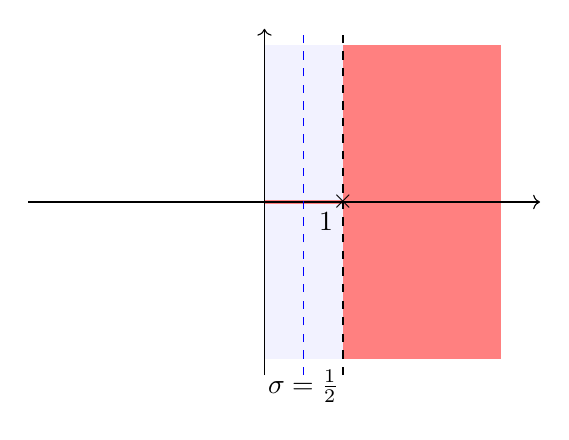
\begin{tikzpicture}
    \fill[blue!5] (0, -2) rectangle (1, 2);
    \draw [red!50, ultra thick] (0, 0) -- (1, 0);
    \fill[red!50] (1, -2) rectangle (3, 2);

    \draw [->] (-3, 0) -- (3.5, 0);
    \draw [->] (0, -2.2) -- (0, 2.2);

    \draw [thick, dashed] (1, -2.2) -- (1, 2.2);


    \node at (1, 0) {\(\times\)};
    \node at (1, 0) [anchor = north east] {\(1\)};

    \draw [blue, dashed] (0.5, -2.2) -- (0.5, 2.2);

    \node at (0.5, -2) [anchor = north] {\(\sigma = \frac{1}{2}\)};
  \end{tikzpicture}
\end{center}

\subsection{Prime number theorem}

Let \(\alpha(s) = \sum \frac{a_n}{n^s}\). Partial summation lets us write \(\alpha(s)\) in terms of \(A(x) = \sum_{n \leq x} a_n\). If \(\sigma > \max (0, \sigma_c)\) then
\[
  \alpha(s) = s \int_1^\infty \frac{A(t)}{t^{s + 1}} dt
\]
This is \emph{Mellin transform}\index{Mellin tranform}.

What about the converse? As a particular case, if \(\alpha(s) = -\frac{\zeta'(s)}{\zeta(s)}\) then \(a_n = \Lambda(n)\) so
\[
  A(x) = \sum_{n \leq x} \Lambda(n) = \psi(x).
\]
The point of analytic number theory is to study Dirichlet series using analytic methods and convert them back to statements about arithmetic functions.

The converse is given by Perron's formula, which roughly says that
\[
  A(x) = \frac{1}{2\pi i} \int_{\sigma - i \infty}^{\sigma + i \infty} \alpha(s) \frac{x^s}{s} ds
\]
for \(\sigma > \max (0, \sigma_c)\).

Before we prove the formula, we see how this leads to prime number theorem. By Perron's formula,
\[
  \psi(x) = \frac{1}{2\pi i} \int_{\sigma - i \infty}^{\sigma + i \infty} -\frac{\zeta'(s)}{\zeta(s)} \frac{x^s}{s} ds
\]
for \(\sigma > 1\).

We see that the integrand has two poles, on at the origin and the other at \(1\). Our first attempt would be to integrate to the right of the critical line as there is no singularity.
\begin{center}
  \begin{tikzpicture}
    \draw [->] (-3, 0) -- (3, 0);
    \draw [->] (0, -2.2) -- (0, 2.2);

    \draw [dashed] (1, -2.2) -- (1, 2.2);

    \node at (0, 0) {\(\times\)};
    \node at (1, 0) {\(\times\)};

    \draw[->, blue, thick] (1.5, 2) -- (1.5, -2) -- (2.5, -2) -- (2.5, 2) -- (1.5, 2);

    \node at (1, 0) [anchor=north east] {\(1\)};
  \end{tikzpicture}
\end{center}

However we quickly run into problems. As the integrand is holomorphic in this region, by Cauchy's theorem \(\psi(x)\) equals to the contribution of the other segments (up to a sign). The best we can do is \(\psi(x) = O(x^{1 + \varepsilon})\), which, in view of what we have done, totally trivial. Thus we can't simply consider a contour in \(\sigma > 1\).

Instead we have to cross the critial line, whih gives \(O(x^{1 - \varepsilon})\), which is what we need. But now we need to understand \(\zeta\) on/to the left of the critial line.

\begin{center}
  \begin{tikzpicture}
    \draw [->] (-3, 0) -- (3, 0);
    \draw [->] (0, -2.2) -- (0, 2.2);

    \draw [dashed] (1, -2.2) -- (1, 2.2);

    \node at (0, 0) {\(\times\)};
    \node at (1, 0) {\(\times\)};

    \draw[->, blue, thick] (1.5, 2) -- (1.5, -2) -- (0.9, -2) -- (0.9, 2) -- (1.5, 2);

    \node at (1, 0) [anchor=north east] {\(1\)};
  \end{tikzpicture}
\end{center}

We can summarise this intuition with the slogan ``prime number theorem is equivalent to the statment that there is no zeroes on \(\sigma = 1\)''.

\begin{lemma}
  If \(\sigma_0 > 0\) then
  \[
    \frac{1}{2\pi i} \int_{\sigma_0 - iT}^{\sigma_0 + iT} \frac{y^s}{s} ds =
    \begin{cases}
      1 & y > 1 \\
      0 & y < 1
    \end{cases}
    + O(\frac{y^{\sigma_0}}{T |\log y|})
  \]
\end{lemma}
Note that we omit the case \(y = 1\).

\begin{proof}
  Use a rectangular contour that lies either to the left or to the right of the line \(\sigma = \sigma_0\) depending on \(y\), which then determines whether the residue at \(0\) is picked up. The details are left as an exercise.
\end{proof}
This gives a way to express indicator function in integral form.

\begin{theorem}[Perron's formula]\index{Perron's formula}
  Suppose \(\alpha(s) = \sum \frac{a_n}{n^s}\) is absolutely convergent for \(\sigma > \sigma_a\). If \(\sigma_0 > \max (0, \sigma_a)\) and \(x\) is not an integer then
  \begin{align*}
    \sum_{n < x} a_n
    &= \frac{1}{2 \pi i} \int_{\sigma_0 - iT}^{\sigma_0 + iT} \alpha(s) \frac{x^s}{s} ds \\
    &+ O(\frac{2^{\sigma_0}x}{T} \sum_{\frac{x}{2} < n < 2x} \frac{|a_n|}{|x - n|} + \frac{x^{\sigma_0}}{T} \sum_{n = 1}^\infty \frac{|a_n|}{n^{\sigma_0}}).
  \end{align*}
\end{theorem}

\begin{proof}
  Since \(\sigma_0 > 0\) we can write
  \[
    1_{n < x}
    = \frac{1}{2\pi i} \int_{\sigma_0 - iT}^{\sigma_0 + iT} \frac{(x/n)^s}{s} ds + O(\frac{(x/n)^{\sigma_0}}{T |\log \frac{x}{n}|})
  \]
  so
  \begin{align*}
    \sum_{n < x} a_n
    &= \sum_n a_n 1_{n < x} \\
    &= \frac{1}{2\pi i} \sum_n a_n \int_{\sigma_0 - iT}^{\sigma_0 + iT} \frac{(x/n)^s}{s} ds + \underbrace{O(\frac{x^{\sigma_0}}{T} \sum_n \frac{|a_n|}{n^{\sigma_0} |\log \frac{x}{n}|})}_E \\
    &= \frac{1}{2\pi i} \int_{\sigma_0 + iT}^{\sigma_0 - iT} \frac{x^s}{s} \sum_n \frac{a_n}{n^s} ds + E \quad \text{absolute convergence} \\
    &= \frac{1}{2 \pi i} \int_{\sigma_0 - iT}^{\sigma_0 + iT} \alpha(s) \frac{x^s}{s} ds + E
  \end{align*}
  For the error term \(E\), there is
  \begin{enumerate}
  \item contribution from \(n \leq \frac{x}{2}\) or \(n \geq 2x\), where \(|\log \frac{x}{n}| \gg 1\), is
    \[
      \ll \frac{x^{\sigma_0}}{T} \sum_n \frac{|a_n|}{n^{\sigma_0}}.
    \]
  \item contribution from \(\frac{x}{2} < n < 2x\), we write
    \[
      |\log \frac{x}{n}| = |\log (1 + \frac{n - x}{x})|
    \]
    and \(|\log (1 + \delta)| \asymp |\delta|\) uniformly for \(- \frac{1}{2} \leq \delta \leq 1\). So
    \[
      \frac{x^{\sigma_0}}{T} \sum_{\frac{x}{2} < n < 2x} \frac{|a_n|}{n^{\sigma_0} |\log \frac{x}{n}|}
      \ll \frac{x^{\sigma_0}}{T} \sum_{\frac{x}{2} < n < 2x} \frac{|a_n| x}{n^{\sigma_0} |x - n|}
      \ll \frac{2^{\sigma_0}}{T} \sum_{\frac{x}{2} < n < 2x} \frac{|a_n| x}{|x - n|}
    \]
  \end{enumerate}
\end{proof}

We will now prove a strong form of the prime number theorem, assuming
\begin{enumerate}
\item there exists \(c > 0\) such that if \(\sigma > 1 - \frac{c}{\log (|t| + 4)}\) and \(|t| \geq \frac{7}{8}\) then \(\zeta(s) \neq 0\) and
  \[
    \frac{\zeta'(s)}{\zeta(s)} \ll \log (|t| + 4).
  \]
\item \(\zeta(s) \neq 0\) for \(\frac{8}{9} \leq \sigma \leq 1, |t| \leq \frac{7}{8}\).
\item Whenever \(|t| \leq \frac{7}{8}\) and
  \[
    1 - \frac{c}{\log (|t| + 4)} < \sigma \leq 2
  \]
  have
  \[
    \frac{\zeta'(s)}{\zeta(s)} = - \frac{1}{s - 1} + O(1).
  \]
\end{enumerate}

\begin{center}
  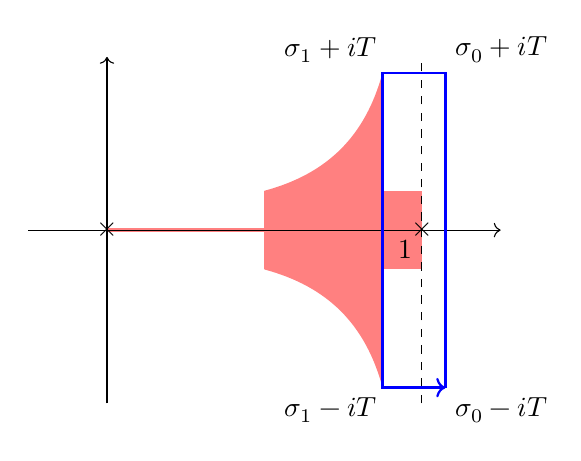
\begin{tikzpicture}
    \draw [red!50, ultra thick] (0, 0) -- (2, 0);
    \fill [red!50] (2, -0.5) rectangle (4, 0.5);

    \path [fill=red!50] (2, 0.5) to [bend right=30] (3.5, 2) -- (3.5, -2) to [bend right=30] (2, -0.5) -- (2, 0.5);

    \draw [->] (-1, 0) -- (5, 0);
    \draw [->] (0, -2.2) -- (0, 2.2);

    
    \draw [dashed] (4, -2.2) -- (4, 2.2);

    \node at (0, 0) {\(\times\)};
    \node at (4, 0) {\(\times\)};
    
    \draw[->, blue, thick] (4.3, -2) -- (4.3, 2) -- (3.5, 2) -- (3.5, -2) -- (4.3, -2);

    \node at (4, 0) [anchor=north east] {\(1\)};
    \node at (4.3, -2) [anchor=north west] {\(\sigma_0 - iT\)};
    \node at (3.5, -2) [anchor=north east] {\(\sigma_1 - iT\)};
    \node at (4.3, 2) [anchor=south west] {\(\sigma_0 + iT\)};
    \node at (3.5, 2) [anchor=south east] {\(\sigma_1 + iT\)};

  \end{tikzpicture}
\end{center}

\begin{theorem}[prime number theorem]\index{prime number theorem}
  There exists \(c > 0\) such that
  \[
    \psi(x) = x + O(\frac{x}{\exp(c \sqrt{\log x})}).
  \]
  In particular \(\psi(x) \sim x\).
\end{theorem}

This error is better than \(\frac{x}{\log x}\) but worse than \(x^{1 - \varepsilon}\) for any \(\varepsilon > 0\), which is precisely because we can't find an absolute bound on the zero-free region near the critical line.

\begin{proof}
  Assume that \(x = N + \frac{1}{2}\) for some \(N\). By Perron's formula, for any \(1 < \sigma_0 \leq 2\),
  \begin{align*}
    \psi(x)
    &= \sum_{n \leq x} \Lambda(n) \\
    &= \frac{1}{2\pi i} \int_{\sigma_0 - iT}^{\sigma_0 + iT} - \frac{\zeta'(s)}{\zeta(s)} \frac{x^s}{s} ds \\
    &+ O(\underbrace{\frac{x}{T} \sum_{\frac{x}{2} < n < 2x} \frac{\Lambda(n)}{|x - n|}}_{R_1} + \underbrace{\frac{x^{\sigma_0}}{T} \sum_{n = 1}^\infty \frac{\Lambda(n)}{n^{\sigma_0}}}_{R_2})
  \end{align*}
  In the error term,
  \[
    R_1
    \ll \log x \cdot \frac{x}{T} \sum_{\frac{x}{2} < n < 2x} \frac{1}{|x - n|}
    \ll \log x \cdot \frac{x}{T} \sum_{1 \leq m \leq 4x} \frac{1}{m}
    \ll \frac{x}{T} (\log x)^2
  \]
  and using assumption 3,
  \[
    R_2
    \ll \frac{x^{\sigma_0}}{T} \frac{1}{|\sigma_0 - 1|}
    \ll \frac{x}{T} \log x
  \]
  if \(\sigma_0 = 1 + \frac{1}{\log x}\).

  Let \(C\) be the rectangular contour with vertices \(\{\sigma_0 \pm iT, \sigma_1 \pm iT\}\) where \(\sigma_1 < 1\) is to be chosen later. Then
  \[
    \frac{1}{2\pi i} \int_C - \frac{\zeta'(s)}{\zeta(s)} \frac{x^s}{s} ds = x
  \]
  by residue theorem and assumption 1 and 2.

  Remains to bound the other components of the integral.
  \[
    \int_{\sigma_0 + iT}^{\sigma_1 + iT} - \frac{\zeta'(s)}{\zeta(s)} \frac{x^s}{s} ds
    \ll \log T \int_{\sigma_0}^{\sigma_1} \frac{x^u}{T} du
    \ll \frac{\log T}{T} x^{\sigma_1} (\sigma_1 - \sigma_0) \ll \frac{x}{T}
  \]
  where the last step is because we assumed \(\sigma_1 = 1 - \frac{c}{\log T}\) (?)

  For the other term,
  \begin{align*}
    \int_{\sigma_1 - iT}^{\sigma_1 + iT} - \frac{\zeta'(s)}{\zeta(s)} \frac{x^s}{s} ds
    &\ll \log T \int_{\sigma_1 - iT}^{\sigma_1 - iT} \frac{x^u}{u} du + \int_{\sigma_1 - iT}^{\sigma_1 + iT} x^{\sigma_1} \frac{1}{|\sigma_1 - 1|} \\
    &\ll x^{\sigma_1} \log T + \frac{x^{\sigma_1}}{1 - \sigma_1} \\
    &\ll x^{\sigma_1} \log T
  \end{align*}

  Thus
  \begin{align*}
    \psi(x)
    &= x + O(\frac{x}{T} (\log x)^2 + x^{1 - \frac{c}{\log T}} (\log T)) \\
    &= x + O(\frac{x}{\exp(c \sqrt{\log x})}) \quad \text{if } T = \exp(c \sqrt{\log x})
  \end{align*}
  If you are curious how we chose \(T\), it is the same trick as in chapter 1: want to have \(\frac{x}{T} \approx x^{1 - \frac{c}{\log T}}\) so
    \[
      \log T \approx \frac{\log x}{\log T},
    \]
    i.e.\ \(\log T \approx \sqrt{\log x}\).
\end{proof}

\subsection{Zero-free region}

Firstly, near \(s = 1\), things are easy because of the pole.

\begin{theorem}
  If \(\sigma > \frac{1 + t^2}{2}\) then \(\zeta(s) \neq 0\). In particular, \(\zeta(s) \neq 0\). If \(\frac{8}{9} \leq \sigma \leq 1, |t| \leq \frac{7}{8}\).

  Also
  \begin{align*}
    \zeta(s) &= \frac{1}{s - 1} + O(1) \\
    - \frac{\zeta'(s)}{\zeta(s)} &= \frac{1}{s - 1} + O(1)
  \end{align*}
  uniformly in \(\frac{8}{9} \leq \sigma \leq 1, |t| \leq \frac{7}{8}\).
\end{theorem}

\begin{proof}
  Recall that
  \[
    \zeta(s) = \frac{s}{s - 1} + s \int_1^\infty \frac{\{u\}}{u^{s + 1}} du
  \]
  so
  \[
    \Big| \zeta(s) - \frac{s}{s - 1} \Big| \leq |s| \int_1^\infty \frac{1}{u^{\sigma + 1}} du \leq \frac{|s|}{\sigma}
    \]
    so if \(\sigma > |s - 1|\), \(\zeta(s) \neq 0\), i.e.\ if \(\sigma < \frac{1 + t^2}{2}\). Also
    \[
      |\zeta(s) - \frac{1}{s - 1}| \leq 1 + |s| \int_1^\infty \frac{1}{u^{\sigma + 1}} du = O(1)
    \]
    so same holds for \(- \frac{\zeta'}{\zeta}\), by general theory of holomorphic functions.
\end{proof}

For \(|t|\) large, we need a different idea. How do we show that there aren't zeros on \(\sigma = 1\)? Suppose there is a zero, of order \(m\), at \(1 + it\). Then
\[
  - \frac{\zeta'}{\zeta} (1 + \delta + it) \sim \frac{m}{\delta}
\]
so
\[
  \sum \frac{\Lambda(n)}{n^{1 + \delta + it}} \sim -\frac{m}{\delta}.
\]
Absolute value of LHS
\[
  \leq \sum \frac{\Lambda(n)}{n^{1 + \delta}}
  = - \frac{\zeta'}{\zeta} (1 + \delta) \sim \frac{1}{\delta}
\]
so this shows \(m \leq 1\). If there is a zero, it is a simple zero.

This also tells us
\[
  \sum_p \frac{\log p}{p^{1 + \delta}} e^{i t \log p} \sim - \sum \frac{\log p}{p^{1 + \delta}}
\]
so
\[
  \cos (t \log p) \approx -1
\]
for almost all \(p\), so \(p^{it} \approx -1, p^{2it} \approx 1\) for almost all \(p\), so there exists a pole at \(1 + 2i t\), which is a contradiction.

We now present a rigorous proof. Before that we need to take a detour in complex analysis.

\begin{lemma}[Borel-Carathéodory lemma]\index{Borel-Carathéodory lemma}
  If \(f\) is holomorphic on \(|z| \leq R\) and \(f(0) = 0\). If \(\Re f(z) \leq M\) for all \(|z| \leq R\), then for any \(r < R\),
  \[
    \sup_{|t| \leq r} (|f(z)|, |f'(z)|) \ll_{r, R} M.
  \]
\end{lemma}
If we replace \(\Re f(z)\) by \(|f(z)|\) then this is just maximum value principle.

\begin{proof}
  Let
  \[
    g(z) = \frac{f(z)}{z (2M - f(z))}.
  \]

  This is holomorphic in \(|z| \leq R\). If \(|z| = R\) then
  \[
    |2M - f(z)| \geq |f(z)|
  \]
  and so
  \[
    |g(z)| \leq \frac{|f(z)|}{R |f(z)|} \leq \frac{1}{R}.
  \]
  So for all \(|z| \leq r < R\), by maximum modules,
  \[
    |g(z)| = \frac{|f(z)|}{|z| |2m - f(z)|} < \frac{1}{R}
  \]
  so
  \[
    R |f(z)| \leq r |2M - f(z)| \leq 2M r + r |f(z)|
  \]
  so
  \[
    |f(z)| \leq \frac{2M r}{R - r} \ll M.
  \]

  For \(f'(z)\), we use Cauchy's formula
  \[
    f'(z) = \frac{1}{\pi i} \int_{|w| = r'} \frac{f(w)}{(z - w)^2} dw
  \]
  for \(r < r' < R\). (coefficient 2?)
\end{proof}

\begin{lemma}
  If \(f\) is holomorphic on a domain including \(|z| \leq 1\), \(|f(z)| \leq M\) in that disc, and \(f(0) \neq 0\). If \(0 < r < R < 1\) then for \(|z| \leq r\)
  \[
    \frac{f'}{f} (z) = \sum_{k = 1}^K \frac{1}{z - z_k} + O_{r, R} (\log \frac{M}{|f(0)|})
  \]
  where \(z_k\) ranges over all zeros of \(f\) in \(|z| \leq R\).
\end{lemma}
c.f. fundamental theorem of algebra, and holomorphicity. This depends crucially on \(\C\) being algebraically closed.

\begin{proof}
  Suppose wlog \(f(0) = 1\). Say first there are no zeros. Consider \(h(z) = \log f(z)\) and
  \[
    \Re h(z) = \log |f(z)| \leq \log M
  \]
  so by Borel-Carathéodory lemma,
  \[
    |h'(z)| = |\frac{f'}{f(z)}| \ll \log M
  \]
  so done.

  In general, we define an auxillary function \(g\) with no zeros. Let
  \[
    g(z) = f(z) \prod_{k = 1}^K \frac{R^2 - z \conj z_k}{(z - z_k) R}.
  \]
  The \(k\)th factor has a pole at \(z = z_k\) and on \(|z| = R\), has modulus \(1\) so on \(|z| \leq R\), \(|g(z)| \leq M\). In particular, \(|g(0)| = \prod_{k = 1}^K \frac{R}{|z_k|} \leq M\). Now let
  \[
    h(z) = \log \frac{g(z)}{g(0)}
  \]
  and
  \[
    \Re h(z) = \log |g(z)| - \log |g(0)| \leq \log M
  \]
  for \(|z| \leq R\). By Borel-Carathéodory lemma,
  \[
    |h'(z)| = |\frac{f'}{f} (z) - \sum_{k = 1}^K \frac{1}{z - z_k} + \sum_{k = 1}^K \frac{1}{z - R^2/\conj z_k} \ll \log M
  \]
  so
  \[
    \frac{f'}{f} (z) = \sum_{k = 1}^K \frac{1}{z - z_k} - \sum_{k = 1}^K \frac{1}{z - R^2/\conj z_k} + O(\log M)
  \]
  and if \(|z| \leq r\),
  \[
    |z - \frac{R^2}{\conj z_k}| \geq \frac{R^2}{z_k} - |z| \geq R - r \gg 1
  \]
  and \(K \ll \log M\).
\end{proof}

\begin{corollary}
  If \(|t| \geq \frac{7}{8}\) and \(\frac{5}{6} \leq \sigma \leq 2\) then
  \[
    \frac{\zeta'}{\zeta}(s) = \sum_\rho \frac{1}{s - \rho} + O(\log |t|)
  \]
  where \(\rho\) is over all zeros in
  \[
    |\rho - (\frac{3}{2} + it)| \leq \frac{5}{6}.
  \]
\end{corollary}

\begin{theorem}
  There exists \(c > 0\) such that \(\zeta(s) \neq 0\) if \(\sigma \geq 1 - \frac{c}{\log t}\).
\end{theorem}

\begin{proof}
  Assume \(\zeta(\rho) = 0\) where \(\rho = \sigma + it\). Let \(\delta > 0\) be chosen later.
  \[
    \frac{\zeta'}{\zeta} (1 + \delta + i t)
    = \frac{1}{1 + \delta + it - \rho} + \sum_{\rho' \neq \rho} \frac{1}{1 + \delta + it - \rho'} + O(\log t)
  \]
  (assuming that \(\sigma\) is sufficiently close to \(1\)). Then
  \begin{align*}
    \Re \frac{\zeta'}{\zeta} (1 + \delta + i t)
    &= \Re \frac{1}{1 + \delta + it - \rho} + \Re \sum_{\rho' \neq \rho} \frac{1}{1 + \delta + it - \rho'} + O(\log t) \\
    &= \frac{1}{1 + \delta - \sigma} + O(\log t) + (> 0)
  \end{align*}
  since \(\Re \rho' \leq 1\), \(\Re \frac{1}{1 + \delta + it - \rho'} > 0\). Thus
  \[
    \Re \frac{\zeta'}{\zeta} (1 + \delta + i t)
    > \frac{1}{1 + \delta - \sigma} + O(\log t)
  \]
  Similarly
  \[
    \Re \frac{\zeta'}{\zeta} (1 + \delta + 2 it) > O(\log t).
  \]
  Also
  \[
    \frac{\zeta'}{\zeta} (1 + \delta) = - \frac{1}{\delta} + O(1).
  \]

  Here comes the clever bit:
  \begin{align*}
    \Re(-3 \frac{\zeta'}{\zeta} (1 + \delta) - 4 \frac{\zeta'}{\zeta} (1 + \delta + it) - \frac{\zeta'}{\zeta} (1 + \delta + 2it))
    &< \frac{3}{\delta} - \frac{4}{1 + \delta - \sigma} + O(\log t)
      \tag{\dagger}
  \end{align*}
  As \(\delta \to 0\), \(\dagger\) is going to be negative. On the other hand, it is a a Dirichlet series
  \begin{align*}
    \dagger
    &= \Re( 3 \sum_n \frac{\Lambda(n)}{n^{1 + \delta}} + 4 \sum_n \frac{\Lambda(n)}{n^{1 + \delta + it}} + \sum_n \frac{\Lambda(n)}{n^{1 + \delta + 2it}} ) \\
    &= \sum_n \frac{\Lambda(n)}{n^{1 + \delta}} (3 + 4 \cos (t \log n) + \cos (2t \log n))
  \end{align*}
  Note
  \[
    3 + 4 \cos \theta + \cos (2\theta) = 2 (1 + \cos \theta)^2 \geq 0
  \]
  so \(\dagger \geq 0\).

  So
  \[
    \frac{3}{\delta} > \frac{4}{1 + \delta - \sigma} + O(\log t).
  \]
  Choose \(\delta = \frac{C}{\log t}\) for large enough \(C\), so get a contradiction if \(\sigma \geq 1 - \frac{c}{\log t}\) for some \(c > 0\).( so
  \[
    \frac{4}{1 + \delta - \sigma} < \frac{10}{\delta}
  \]
  so \(\sigma \geq 1 - \frac{c}{\log t}\).)
\end{proof}

It's essentially what we are able to do nowadays. Best known to date is
\[
  \sigma \geq 1 - \frac{c (\log \log t)^{1/3}}{(\log t)^{2/3}}.
\]

\begin{lemma}
  If \(\sigma > 1 - \frac{c}{2 \log t}\) and \(|t| \geq \frac{7}{8}\) then
  \[
    |\frac{\zeta'}{\zeta}(s)| \ll \log t.
  \]
\end{lemma}

\begin{proof}
  Let \(s_1 = 1 + \frac{1}{\log t} + it = \sigma_1 + it\). Here
  \[
    |\frac{\zeta'}{\zeta}(s_1)|
    \ll \sum_{n = 1}^\infty \frac{\Lambda(n)}{n^{\sigma_1}}
    \ll \frac{1}{\sigma_1 - 1}
    \ll \log t.
  \]
  Use the corollary
  \[
    \frac{\zeta'}{\zeta}(s_1) = \sum_\rho \frac{1}{s_1 - \rho} + O(\log t)
  \]
  so therefore
  \[
    \Re \sum_\rho \frac{1}{s_1 - \rho} \ll \log t.
  \]
  Now if \(s = \sigma + it\), where \(\sigma > 1 - \frac{c}{2 \log t}\) then
  \[
    \frac{\zeta'}{\zeta}(s) - \frac{\zeta'}{\zeta}(s_1)
    = \sum_\rho (\frac{1}{s - \rho} - \frac{1}{s_1 - \rho}) + O(\log t)
  \]
  Also \(|s - \rho| \asymp |s_1 - \rho|\) so
  \[
    |\frac{1}{s - \rho} - \frac{1}{s_1 - \rho}|
    \ll \frac{1}{|s_1 - \rho|^2 \log t}
    \ll \Re \frac{1}{s_1 - \rho}
  \]
  as \(\Re \frac{1}{z} = \frac{\Re z}{|z|^2}\). Then
  \[
    \sum_\rho |\frac{1}{s - \rho} - \frac{1}{s_1 - \rho}|
    \ll \Re \sum_\rho \frac{1}{s_1 - \rho}
    \ll \log t.
  \]
\end{proof}

Assuming the Riemann hypothesis, we can show
\[
  \psi(x) = x + O(x^{1/2} (\log x)^2).
\]
See example sheet. Using partial summation, we can deduce that
\[
  \pi(x) = \operatorname{Li} (x) + O_\varepsilon(x^{1/2 + \varepsilon})
\]
where
\[
  \operatorname{Li} (x)
  = \int_2^x \frac{1}{\log t} dt
  = \frac{x}{\log x} + O(\frac{x}{(\log x)^2}).
\]
Thus if we write \(\pi(x) = \frac{x}{\log x} + E(x)\) then
\[
  E(x) \gg \frac{x}{(\log x)^2}
\]
just because of \(\operatorname{Li}\).

\subsection{Error terms}

Indeed if we assume Riemann hypothesis then we could get the error term as above. Can we do better? In this section we will show that
\[
  |\psi(x) - x| \gg x^{1/x}
\]
``often''. Thus apart from the factor \((\log x)^2\) we are getting the best possible error term. The reason is basically that there are many zeros of \(\zeta\) on the critical line. Actually, we will show that
\[
  \psi(x) = x + \Omega_{\pm} (x^{1/2}),
\]
i.e.
\begin{align*}
  \limsup_{x \to \infty} \frac{\psi(x) - x}{x^{1/2}} &> 0 \\
  \liminf_{x \to \infty} \frac{\psi(x) - x}{x^{1/2}} &< 0
\end{align*}

For contradiction, suppose that \(\psi(x) - x \leq cx^{1/2}\) for all large \(x\), so \(cx^{1/2} - \psi(x) = x \geq 0\). Take Mellin transform of this,

\begin{lemma}[Landau]
  Let \(A(x)\) be intergrable and boundedon any finite interval and \(A(x) \geq 0\) for all \(x \geq X\). Let
  \[
    \sigma_c = \inf \{\sigma: \int_X^\infty A(x) x^{-\sigma} dx < \infty\}.
  \]
  Then if
  \[
    F(s) = \int_1^\infty A(x) x^{-s} dx
  \]
  then \(F\) is analytic for \(\Re s > \sigma_c\) and \emph{not} at \(s = \sigma_c\).
\end{lemma}
General fact about poles of Dirichlet series with positive coefficients.

\begin{proof}
  Divide integrand into \([1, X]\) and \([X, \infty)\) , corresponding partition of \(F = F_1 + F_2\). \(F_1\) is entire. If \(\Re s > \sigma_c\), the integral converges absolutely so \(F_2\) is analytic.

  By contradiction, suppose \(F_2\) is analytic at \(s = \sigma_c\). Write \(F_2\) as a Taylor series around \(\sigma_c + 2\)
  \[
    F_2(s) = \sum_{k = 0}^\infty c_k (s - \sigma_c - 1)^k
  \]
  where
  \[
    c_k = \frac{F_2^{(k)}(\sigma_c + 1)}{k!} = \frac{1}{k!} \int_x^\infty A(x) (-\log x)^k x^{- \sigma_c - 1} dx.
  \]
  This power series has a radius of convergence, which must be \(1 + \delta\) for some \(\delta > 0\). So
  \[
    F_2(s) = \sum_{k = 0}^\infty \frac{(1 - \sigma_c - s)^k}{k!} \int_x^\infty A(x) (\log x)^k x^{-1 - \sigma_c} dx
  \]
  Evaluate the series at \(s = \sigma_c - \frac{\delta}{2}\), we can intercahnge the integral and summation so
  \[
    F_2(\sigma_c - \frac{\delta}{2})
    = \int_x^\infty A(x) x^{-1 - \sigma_c} \exp((1 + \sigma_c - s) \log x) dx
    = \int_x^\infty A(x) s^{-s} dx
  \]
  so the integral converges at \(\sigma_c - \frac{\delta}{2}\), contradicting the definition of \(\sigma_c\).
\end{proof}

\begin{theorem}[Landau]
  If \(\sigma_0\) is the supremum of the real parts of
  \[
    \{\rho: \zeta(\rho) = 0\}
  \]
  then
  \begin{enumerate}
  \item for any \(\sigma < \sigma_0\),
    \[
      \psi(x) - x = \Omega_\pm (x^\sigma),
    \]
  \item if there is zero \(\rho\) with \(\sigma = \sigma_0\) then
    \[
      \psi(x) - x = \Omega_\pm (x^{\sigma_0}).
    \]
  \end{enumerate}
\end{theorem}

\begin{corollary}
  (Assuming there is a zero with \(\sigma = \frac{1}{2}\), which is indeed true)
  \[
    \psi(x) - x = \Omega_\pm (x^{1/2}).
  \]
\end{corollary}
Proof by splitting into cases Riemann hypothesis is true/false.

\begin{corollary}
  \label{cor:RH equivalent to bound on PNT}
  Riemann hypothesis is equivalent to
  \[
    \psi(x) = x + O(x^{1/2 + o(1)}).
  \]
\end{corollary}

\begin{proof}
  Let \(c > 0\) be chosen later and suppose that \(\psi(x) - x \leq c x^\sigma\) for all \(x \geq X\). Consider
  \[
    F(s) = \int_1^\infty (cx^\sigma - \psi(x) + x) x^{-s - 1} dx.
  \]
  Recall that by partial summation, for \(\Re s > 1\),
  \begin{align*}
    \frac{\zeta'}{\zeta}(s) &= -s \int_1^\infty \psi(x) x^{-s - 1} dx \\
    \int_1^\infty x^{-s} &= \frac{1}{s - 1}
  \end{align*}
  so
  \[
    F(s) = \frac{c}{s - \sigma} + \frac{\sigma'(s)}{s \zeta(s)} + \frac{1}{s - 1}.
  \]
  This has a pole at \(s = \sigma\) and is analytic for \(\Re s > \sigma\). By Landau's lemma, in fact this integral converges for all \(s\) with \(\Re s > \sigma\). This proves 1 because if \(\sigma < \sigma_0\) then there is a zero of \(\zeta\) with \(0 < \Re \rho < \sigma_0\) and at \(\rho\) \(F\) has a singularity since \(\rho \notin \R\).

  Suppose there is \(\rho = \sigma_0 + it_0\). Repeat the above with \(\sigma = \sigma_0\). Consider instead
  \[
    G(s) = F(s) + \frac{e^{i\theta} F(s + it_0) + e^{-i\theta} F(s - it_0)}{2}
  \]
  where \(\theta \in \R\) is to be chosen later. \(G(s)\) is still analytic for \(\Re s > \sigma\), and has a pole at \(s = \sigma_0\). From \(F(s)\), have residue. From \(F(s + it_0)\), have residue \(\frac{m}{\rho}\) where \(m\) is the order of \(\rho\). From \(F(s - it_0)\) have residue \(\frac{m}{\conj \rho}\). So \(G(s)\) has a pole at \(s = \sigma_0\) with residue
  \[
    c + \frac{e^{i\theta} m}{2 \rho} + \frac{e^{-i\theta}m}{2 \conj \rho} = c - \frac{m}{|\rho|}
  \]
  by choosing appropriate \(\theta\). In particular if \(c < \frac{m}{|\rho|}\) then this residue is negative. As \(s \to \sigma_0\) from right along \(\R\), \(G(s) \to - \infty\). But for \(\Re s > \sigma_0\),
  \[
    G(s) = \int_1^\infty (c x^{\sigma_0} - \psi(x) = x) x^{-s - 1} \underbrace{(1 + \frac{e^{i\theta} x^{-it_0}}{2} +  \frac{e^{-i\theta} x^{it_0}}{2})}_{1 + \cos (\theta - t_0 \log x) \geq 0} dx
  \]
  so splitting the integral into \([1, X]\) and \([X, \infty)\), \(G(s) = G_1(s) + G_2(s)\) where \(G_1\) is entire and \(G_2(s) \geq 0\) as \(s \in \R, \Re s > \sigma_0\). Absurd. This proves
  \[
    \psi(x) - x = \Omega_+(x^\sigma).
  \]
  \(\Omega_-\) is the same.
\end{proof}

\subsection{Functional equation}

Recall that for \(\sigma > 0\), we defined
\[
  \zeta(s) = 1 + \frac{1}{s - 1} - s \int_1^\infty \frac{\{t\}}{t^{s + 1}} dt.
\]
How does it behave in the negative half plane?

First define \(f(t) = \frac{1}{2} - \{t\}\), so
\[
  \zeta(s) = \frac{1}{s - 1} + \frac{1}{2} + s \int_1^\infty \frac{f(t)}{t^{s + 1}} dt
\]
which actually converges when \(\sigma > -1\). To see this, let
\[
  F(x) = \int_0^x f(t) dt
\]
so
\[
  \int_X^Y \frac{f(t)}{t^{s + 1}} dt
  = \frac{F(t)}{t^{s + 1}} \Big|_X^Y + (s + 1) \int_X^Y \frac{F(t)}{t^{s + 1}} dt
\]
and note that \(F(t)\) is bounded (as seen from the graph of \(f\)). Therefore
\[
  \int_1^\infty \frac{f(t)}{t^{s + 1}} dt
\]
converges when \(\sigma > -1\). We can take this as the definition of \(\zeta(s)\) for \(\sigma > -1\). At this point, we can do (perfectly sensible) things such as
\[
  \zeta(0) = -\frac{1}{2} = 1 + 1 + 1 + \cdots
\]
It is evident that we by iterating the process we may extend \(\zeta(s)\) to arbitrary \(\sigma < 0\), but there is a more elegant way to do this. First let's simplify the integral. Note that for \(-1 < \sigma < 0\),
\[
  s \int_0^1 \frac{f(t)}{t^{s + 1}}
  = \frac{s}{2} \int_0^1 \frac{1}{t^{s + 1}} dt - s \int_0^1 \frac{1}{t^s} dt
  = \frac{1}{2} + \frac{1}{s - 1}
\]
so in the strip \(-1 < \sigma < 0\), have
\[
  \zeta(s) = s \int_0^\infty \frac{f(t)}{t^{s + 1}} dt.
\]
By Fourier analysis, \(f(t)\) has a Fourier seires
\[
  f(t) = \sum_{n = 1}^\infty \frac{\sin (2n \pi t)}{n \pi}
\]
which converges whenver \(t \notin \Z\). In the region \(-1 < \sigma < 0\), we get (by a standard argument exchanging summation and integration)
\begin{align*}
  \zeta(s)
  &= s \int_0^\infty \frac{1}{t^{s + 1}} \sum_{n = 1}^\infty \frac{\sin (2n \pi t)}{n \pi} dt \\
  &= s \sum_{n = 1}^\infty \frac{1}{n\pi} \int_0^\infty \frac{\sin(2n \pi t)}{t^{s + 1}} dt \\
  &= s \sum_{n = 1}^\infty \frac{(2n\pi)^s}{n\pi} \int_0^\infty \frac{\sin y}{y^{s + 1}} dy \quad y = 2n\pi t
\end{align*}
Here
\[
  \sum_{n = 1}^\infty \frac{(2n\pi)^s}{n\pi} = 2^s \pi^{s - 1} \zeta(1 - s)
\]
and
\[
  \int_0^\infty \frac{\sin y}{y^{s + 1}} dy
  = \frac{1}{2i} \left( \int_0^\infty \frac{e^{iy}}{y^{s + 1}} dy - \int_0^\infty \frac{e^{-iy}}{y^{s + 1}} dy \right)
  = - \sin \left( \frac{s\pi}{2} \right) \Gamma(-s)
\]
where
\[
  \Gamma(s) = \int_0^\infty t^{s - 1}e^{-t} dt
\]
for \(\sigma > 0\) is the \emph{gamma function}\index{gamma function}. We do a sanity check that the Dirichlet series and gamma function makes sense in the region.

Let's have a digression about gamma function. The first identity is
\[
  \Gamma(s + 1)
  = \int_0^\infty t^s e^{-t} dt
  = -t^s e^{-t} \big|_0^\infty + s \int_0^\infty t^{s - 1} e^{-t} dt
  = s \Gamma(s).
\]
In particular, since \(\Gamma(1) = 1\),
\[
  \Gamma(n) = (n - 1)!
\]
which generalises factorial\footnote{As a side remark, really we should have \(t^s\) in the integrand in the definition of gamma function so it is more consistent and things look nicer on the whole, at least from a number theory point of view. There were people in the 19th century using this notation but unfortunately a huge literature war ensued and obviously it didn't catch up.}. Also note \(\Gamma(s + 1) = s \Gamma(s)\) allows us to extend \(\Gamma(s)\) to \(\C\) with poles at \(s = 0, -1, -2, \cdots\).

Back to the zeta function. This mean that for \(-1 < \sigma < 0\),
\begin{align*}
  \zeta(s)
  &= s 2^s \pi^{s - 1} \zeta(1 - s) (- \sin \left( \frac{\pi s}{2} \right) \Gamma(-s)) \\
  &= 2^s \pi^{s - 1} \sin \left( \frac{s \pi}{2} \right) \Gamma(1 - s) \zeta(1 - s)
\end{align*}
RHS is defined for all \(\sigma < 0\), so we define
\[
  \zeta(s) = 2^s \pi^{s - 1} \sin \frac{s \pi}{2} \Gamma(1 - s) \zeta(1 - s)
\]
for \(\sigma < 0\). This gives an analytic continuation of \(\zeta(s)\) to the negative half plane. Together with the integral expression for \(\sigma > -1\), this gives a meromorphic zeta function on \(\C\).

\begin{theorem}[functional equation]
  For all \(s \in \C\),
  \[
    \zeta(s) = 2^s \pi^{s - 1} \sin \left( \frac{\pi s}{2} \right) \Gamma(1 - s) \zeta(1 - s).
  \]
\end{theorem}

We can poke around the equation and do some reality check:
\begin{itemize}
\item At \(s = 1\),
  \[
    \zeta(1) = 2 \gamma(0) \zeta(0)
  \]
  and as \(\zeta(0) = -\frac{1}{2}\), \(\Gamma\) has a pole at \(0\), this makes sense.
\item Does \(\zeta(s)\) have any other poles? Since
  \[
    \zeta(s) = \underbrace{2^s \pi^{s - 1} \sin \left( \frac{\pi s}{2} \right)}_{\text{entire}} \underbrace{\Gamma(1 - s) \zeta(1 - s)}_{\text{entire for } \sigma < 0}
  \]
  \(\zeta(s)\) is analytic everywhere in \(\C\) except for a simple pole at \(s = 1\).
\item At \(s = 2\),
  \[
    \zeta(2) = 4 \pi \cdot 0 \cdot \Gamma(-1) \zeta(-1).
  \]
  The zero and pole of \(\Gamma\) at \(-1\) cancels and we get a constant \(\frac{\pi^2}{6}\).
\item At \(s = -1\),
  \[
    \zeta(-1)
    = \frac{1}{2} \cdot \frac{1}{\pi^2} \cdot (-1) \cdot \Gamma(2) \zeta(2)
    = -\frac{1}{12}.
  \]
  Of course to physicists, this implies that
  \[
    -\frac{1}{12} = 1 + 2 + 3 + \cdots
  \]
\end{itemize}

What about zeros of zeta function? At a zero we have
\[
  0 = \zeta(s) = \text{nonzero term} \cdot \sin \left( \frac{\pi s}{2} \right) \Gamma(1 - s) \zeta(1 - s).
\]
If \(\sigma < 1\), \(\zeta(1 - s) \neq 0, \Gamma(1 - s) \neq 0\) except \(s = -2n\) where \(n \in \N\). This is a necessary and sufficient condition so \(\zeta(s)\) has zeros at \(-2, -4, \cdots\). We knew that \(\zeta(s)\) has no zeros for \(\sigma \geq 1\) and \(\sigma = 0\). Thus except for the trivial zeros, \(\zeta(s)\) only has zeros in the critical strip \(0 < \sigma < 1\).

In the region \(0 < \sigma < 1\),
\[
  0 = \zeta(s) = \text{nonzero term} \cdot \underbrace{\Gamma(1 - s)}_{\neq 0} \zeta(1 - s)
\]
so \(\zeta(1 - s) = 0\). Also because \(\zeta(\conj s) = \conj{\zeta(s)}\), zeros appear in quadruples. The dream that they actually come in pairs leads to, of course, the Riemann hypothesis.

Now we can fully justify \cref{cor:RH equivalent to bound on PNT}, which states that Riemann hypothesis is equivalent to
\[
  \psi(x) = x + O(x^{1/2 + o(1)}).
\]

\begin{proof}\leavevmode
  \begin{itemize}
  \item \(\implies\): contour integration
  \item \(\impliedby\): we know if \(\sigma_0 = \sup \{\Re \rho: \zeta(\rho) = 0\}\) then
    \[
      \psi(x) = x + \Omega_\pm (x^\sigma)
    \]
    for all \(\sigma < \sigma_0\). If Riemann hypothesis is false then there exists a zero \(\rho\) with \(0 < \sigma < 1, \sigma \neq \frac{1}{2}\). By symmetry, we have
    \[
      \sigma_0 \geq \max (\sigma, 1 - \sigma) > \frac{1}{2}
    \]
    so
    \[
      \psi(x) = x + \Omega_\pm(x^{\sigma'})
    \]
    where \(\frac{1}{2} < \sigma' < \sigma\).
  \end{itemize}
\end{proof}

\section{Primes in arithmetic progressions}

In this last chapter we will introduce Dirchlet characters and use them to prove Dirichlet's theorem, which says that any arithmetic progression satisfying obviously necessary conditions contains infinitely many primes.

\subsection{Dirichlet characters and \(L\)-functions}

\begin{definition}[Dirichlet character]\index{Dirichlet character}
  Fix \(q \in \N\). A \emph{Dirichlet character} of modulus \(q\) is a group homomorphism \(\chi: (\Z/q\Z)^\times \to \C^\times\).
\end{definition}

\((\Z/q\Z)^\times\) is a finite abelian group of order \(\phi(q)\), so the set of Dirichlet characters of modulus \(q\) forms a finite abelian group of order \(\phi(q)\).

We can also think of \(\chi\) as defining a function \(\chi: \Z \to \C\), given by
\[
  \chi(a) =
  \begin{cases}
    \chi(a \bmod q) & (a, q) = 1 \\
    0 & \text{otherwise}
  \end{cases}
\]
Note that this \(\chi\) is periodic with period \(q\) and is totally multiplicative.

If \(\chi\) is the trivial homomorphism on \((\Z/q\Z)^\times\), we call it the \emph{principal Dirichlet character}\index{Dirichlet character!principal} modulus \(q\) and usually denote it as \(\chi_0\).

\begin{lemma}\leavevmode
  \begin{enumerate}
  \item Let \(\chi\) be a Dirichlet character of modulus \(q\). Then
    \[
      \sum_{a \in (\Z/q\Z)^\times} \chi(a)
      = \sum_{1 \leq a \leq q} \chi(a)
      =
      \begin{cases}
        \phi(q) & \chi = \chi_0 \\
        0 & \chi \neq \chi_0
      \end{cases}
    \]
  \item Let \(a \in (\Z/q\Z)^\times\). Then
    \[
      \sum_\chi \chi(a) =
      \begin{cases}
        \phi(q) & q = 1 \bmod q \\
        0 & a \neq 1 \bmod q
      \end{cases}
    \]
  \end{enumerate}
\end{lemma}
For those of you familiar with representation theory, this is the row and column orthogonality for character table of the abelian group \((\Z/q\Z)^\times\).

\begin{proof}
  We treat 2. If \(a = 1 \bmod q\) then \(\chi(a) = 1\) for all \(\chi\) so
  \[
    \sum_\chi \chi(a) = \sum_\chi 1 = \phi(q).
  \]
  If \(q \neq 1 \bmod q\) then there exists \(\psi: (\Z/q\Z)^\times \to \C^\times\) such that \(\psi(a) \neq 1\). The map \(\chi \mapsto \chi \psi\) is a permutation of the set of Dirichlet characters mod \(q\). Hence
  \[
    \sum_\chi \chi(a)
    = \sum_\chi (\chi \psi) (a)
    = \psi(a) \sum_\chi \chi(a)
  \]
  so \(\sum_\chi \chi(a) = 0\).
\end{proof}

Let \(a \in \Z, (a, q) = 1\). Consider \(1_{x = a \bmod q}: \Z \to \C\). The the lemma says that
\[
  1_{x = a \bmod q} (x) = \frac{1}{\phi(q)} \sum_\chi \chi(a)^{-1} \chi(x).
\]
It follows that
\[
  \sum_{\substack{p \leq x \\ p = a \bmod q}} 1
  = \sum_{p \leq x} 1_{x = a \bmod q}(p)
  = \frac{1}{\phi(q)} \sum_{p \leq x} \sum_\chi \chi(a)^{-1} \chi(p).
\]
Estimating this is closely related to estimating 
\[
  \frac{1}{\phi(q)} \sum_{n \leq x} \sum_\chi \chi(a)^{-1} \chi(n) \Lambda(n)
  = \sum_\chi \frac{\chi(a)^{-1}}{\phi(q)} \sum_{n \leq x} \chi(n) \Lambda(n).
\]
The strategy to prove Dirichlet's theorem is to consider the contribution of each character \(\chi\) separately. We will do this using the \emph{Dirichlet \(L\)-function}\index{Dirichlet \(L\)-function}
\[
  L(s, \chi) = \sum_{n \geq 1} \chi(n) n^{-s}.
\]
This series converges absolutely in the region \(\sigma > 1\) and defines an analytic function there.

\begin{lemma}
  If \(\chi \neq \chi_0\) then \(\sum_{n \geq 1} \chi(n) n^{-s}\) converges in \(\sigma > 0\).
\end{lemma}

\begin{proof}
  Use partial summmation,
  \[
    \sum_{n \leq x} \chi(n) n^{-s} = A(x) x^{-s} - \int_1^x A(t) f'(t) dt
  \]
  where \(A(x) = \sum_{n \leq x} \chi(n)\). Note that by the lemma \(\sum_{1 \leq n \leq q} \chi(n) = 0\) as \(\chi \neq \chi_0\). Hence \(A(n)\) is periodic and \(|A(x)| \leq \phi(q)\) for all \(x\). Thus \(|A(x)x^{-s}| \leq \phi(q) x^{-\sigma}\) and the integral is absolutely convergent.
\end{proof}
Thus \(L(s, \chi)\) is analytic in the same region and in particular does not have a pole at \(s = 1\).

Since \(\chi(n)\) is multiplicative, we have an Euler product identity\index{Euler product}
\[
  L(s, \chi) = \prod_p (1 - \chi(p) p^{-s})^{-1}
\]
valid in the region \(\sigma > 1\). This implies that when \(\chi = \chi_0\),
\[
  L(s, \chi_0) = \zeta(s) \prod_{p \divides q} (1 - p^{-s})
\]
so \(L(s, \chi_0)\) has a meromorphic continuation to all \(s \in \C\) and a simple pole at \(s = 1\). We can show that
\[
  \log L(s, \chi) = \sum_p \sum_{k \geq 1} \chi(p)^k p^{-ks}/k
\]
and hence
\[
  \frac{L'}{L}(s, \chi)
  = \sum_p \sum_{k \geq 1} \chi(p)^k (-\log p) p^{-s}
  = -\sum_{n \geq 1} \chi(n) \Lambda(n) n^{-s}
\]
valid in \(\sigma > 1\).

Fix \(a \in \N, (a, q) = 1\). We combine this with the identity valid for any \(n \in \N\)
\[
  1_{n = a \bmod q} (n) = \frac{1}{\phi(q)} \sum_\chi \chi(a^{-1})\chi(n)
\]
we get
\[
  \sum_{n \geq 1} 1_{n = a \bmod q}(n)  \Lambda(n)n^{-s}
  = - \frac{1}{\phi(q)} \sum_\chi \chi(a^{-1}) \frac{L'(s, \chi)}{L(s, \chi)}
\]
again valid in \(\sigma > 1\).

\subsection{Dirichlet's theorem}

\begin{theorem}
  Given \(q \in \N, (a, q) = 1\), there are infinitely many primes \(p\) such that \(p = a \bmod q\).
\end{theorem}

As \(L(s, \chi_0)\) has a simple pole at \(s = 1\), we can write
\[
  \sum_{n \geq 1} 1_{n = a \bmod q} (n) \Lambda(n) n^{-s}
  = \frac{1}{\phi(q)} \frac{1}{s - 1} + O(1) - \frac{1}{\phi(q)} \sum_{\chi \neq \chi_0} \chi(a^{-1}) \frac{L'(s, \chi)}{L(s, \chi)}.
\]
Assume the unknown term is convergent, so RHS has a pole at \(s = 1\) so diverges there. If there were finitely many prime \(p = a \bmod q\), LHS would be bounded as \(s \to 1\), absurd. Thus to show Dirichlet's theorem it is enough to show that for all \(\chi \neq \chi_0\), \(\frac{L'}{L} (s, \chi)\) is analytic at \(s = 1\). This is equivalent to show that if \(\chi \neq \chi_0\) then \(L(1, \chi) \neq 0\).

\begin{theorem}
  If \(\chi \neq \chi_0\) then \(L(1, \chi) \neq 0\).
\end{theorem}

\begin{proof}
  In \(\sigma > 1\), by choosing a branch of logarithm
  \begin{align*}
    \prod_\chi L(s, \chi)
    &= \exp \sum_\chi \log L(s, \chi) \\
    &= \exp \sum_\chi \sum_p \sum_{k \geq 1} \chi(p)^k p^{-ks}/k \\
    &= \exp \sum_\chi \sum_{n \geq 1} \frac{\chi(n) n^{-s} \Lambda(n)}{\log n} \\
    &= \exp \sum_{n \geq 1} \frac{n^{-s} \Lambda(n)}{\log n} \sum_\chi \chi(n) \quad \text{absolute convergence}
  \end{align*}
  We have
  \[
    \sum_\chi \chi(n) =
    \begin{cases}
      0 & (q, n) > 1 \text{ or } (q, n) = 1 \text{ and } n \neq 1 \bmod q \\
      \phi(q) & n = 1 \bmod q
    \end{cases}
  \]
  so
  \[
    \prod_\chi L(s, \chi)
    = \exp \sum_{\substack{n \geq 1 \\ n = 1 \bmod q}} \frac{n^{-s} \Lambda(n)}{\log n} \phi(q)
  \]
  valid in \(\sigma > 1\). For \(s\) real, \(s > 1\), the exponent is a non-negative real numbur. Thus for \(s \in (1, \infty)\),
  \[
    \prod_\chi L(s, \chi) \in [1, \infty).
  \]
  Note that \(L(s, \chi_0)\) has a simple pole at \(s = 1\). If there are at least two distinct characters \(\psi, \psi'\) of modulus \(q\) such that \(L(1, \psi) = L(1, \psi') = 0\) then \(\prod_\chi L(s, \chi)\) would be analytic in a neighbourhood of \(s = 1\), and vanish at \(s = 1\). This cannot happen so there is at most one character \(\psi\) such that \(L(1, \psi) = 0\).

  Note also that for any \(\chi\),
  \[
    L(1, \conj \chi) = \conj{L(1, \chi)}.
  \]
  If \(L(1, \chi) = 0\) then \(L(1, \conj \chi) = 0\). Hence if \(L(1, \chi) = 0\) then \(\chi = \conj \chi\). In other words, \(\chi\) takes values in \(\{\pm 1\}\). We call such characters \emph{quadratic}\index{Dirichlet character!quadratic},

  Suppose for contradiction there exists a non-principal quadratic character \(\psi: (\Z/q\Z)^\times \to \{\pm 1\}\) such that \(L(1, \psi) = 0\). We consider the product \(L(s, \psi) \zeta(s)\). This function is analytic in \(\sigma > 0\). In \(\sigma > 1\) we have the expressoin
  \[
    L(s, \psi) \zeta(s)
    = \left( \sum_{n \geq 1} \psi(n) n^{-s} \right) \left( \sum_{n \geq 1} n^{-s} \right)
    = \sum_{n \geq 1} r(n) n^{-s}
  \]
  where \(r(n) = \sum_{d \divides n} \psi(d)\). Note that \(r(n)\) is multiplicative and \(r(n) \geq 0\):
  \[
    r(p^k) = \psi(1) + \psi(p) + \dots + \psi(p^k) =
    \begin{cases}
      k + 1 & \psi(p) = 1 \\
      1 & \psi(p) = 0 \text{ or } \psi(p) = -1, k \text{ is even} \\
      0 & \psi(p) = -1, k \text{ is odd}
    \end{cases}
  \]
  Note also that \(r(n^2) \geq 1\) by the same argument.

  We now use Landau's lemma
  \begin{lemma}
    Let \(f(s) = \sum_{n \geq 1} a_n n^{-s}\) where \(a_n\) are non-negative real numbers. Suppose given \(\sigma_0 \in \R\) such that \(f(s)\) is convergent in \(\sigma > \sigma_0\). Suppose that \(f(s)\) admits an analytic continuation to the disk \(\{|s - \sigma_0| < \varepsilon\}\). Then \(f(s)\) is convergent in \(\sigma > \sigma_0 - \varepsilon\).
  \end{lemma}
  Let
  \[
    f(s) = L(\psi, s) \zeta(s) = \sum_{n \geq 1} r(n)n^{-s},
  \]
  valid in \(\sigma > 1\). Then we can use Landau's lemma, together with the fact that \(f(s)\) is analytic in \(\sigma > 0\), to conclude that \(f(s)\) is convergent in \(\sigma > 0\). But
  \[
    f\left(\frac{1}{2}\right)
    = \sum_{n \geq 1} r(n) n^{-1/2} \geq \sum_{n \geq 1} r(n^2)/n 
    \geq \sum_{n \geq 1} \frac{1}{n}
  \]
  and this series diverges, absurd. Thus \(L(1, \psi) \neq 0\).
\end{proof}

\subsection{Zero-free region}

We have proved there are infinitely many primes congruent to \(a\) mod \(q\) if \((a, q) = 1\), using
\[
  -\frac{L'}{L}(s, \chi) = \sum_n \frac{\Lambda(n) \chi(n)}{n^s}.
\]
We want to prove a prime number theorem for such primes. To do this, we'll use Perron's formula just as the case for Riemann zeta function. We need more information about the zeros of \(L(s, \chi)\). (roughly speaking \(L(1, \chi) \neq 0\) is the statement there are infinitely many primes. Specialising to \(\chi = 1\) (Riemann zeta function) we get a pole so it is particularly easy to prove there are infinitely many primes).

Similarities to zero-free region for \(\zeta(s)\), but important difference: \(\zeta(s)\) has a pole at \(s = 1\), while \(L(s, \chi)\) has \emph{no} poles for \(\sigma > 0\) for \(\chi \neq \chi_0\).

Some shorthands: let \(\tau = |t| + 4\). Recall
\begin{lemma}
  If \(f(z)\) is analytic on a region containing \(|z| \leq 1\) and \(f(0) \neq 0\) and \(|f(z)| \leq M\) for \(|z| \leq 1\), then for \(0 < r < R < 1\), for \(|z| \leq r\),
  \[
    \frac{f'}{f}(z) = \sum \frac{1}{z - z_k} + O(\log \frac{M}{|f(0)|})
  \]
  where \(z_k\) ranges over zeros of \(f\) in \(|z| \leq R\).
\end{lemma}

\begin{lemma}
  If \(\chi \neq \chi_0\) and \(\frac{5}{6} \leq \sigma \leq 2\) then
  \[
    \frac{L'}{L}(s, \chi) = \sum_\rho \frac{1}{s - \rho} + O(\log qt)
  \]
  over \(\rho\) with \(|\rho - (\frac{3}{2} + it)| \leq \frac{5}{6}\).
\end{lemma}

\begin{proof}
  Follows from the lemma with \(f(z) = L(z + \frac{3}{2} + it, \chi), R = \frac{5}{6}, r = \frac{2}{3}\). Verify that
  \[
    |f(0)|
    = |L(\frac{3}{2} + it, \chi)|
    = \prod_p \left| 1 - \frac{\chi(p)}{p^{3/2 + it}} \right|
    \geq \prod_p \left( 1+ \frac{1}{p^{3/2}} \right)^{-1}
    \gg 1.
  \]
  By partial summation, if \(F(t) = \sum_{1 \leq n \leq t} \chi(n)\) for \(\sigma > 0\) then
  \[
    L(s, \chi) = s\int_1^\infty \frac{F(t)}{t^{s + 1}} \d t
  \]
  so
  \[
    |L(s, \chi)|
    \ll |s| q \int_1^\infty \frac{1}{t^{\sigma + 1}} \d t
    \ll q \tau.
  \]
\end{proof}

\begin{theorem}
  Let \(\chi\) be a non-quadratic character\index{Dirichlet character!quadratic}. Then there is an absolute constant \(c > 0\)  such that \(L(s, \chi) \neq 0\) if \(\sigma > 1 - \frac{c}{\log (q\tau)}\)
\end{theorem}

\begin{proof}
  Since
  \[
    L(s, \chi_0) = \zeta(s) \prod_{p \divides q} (1 - p^{-s}),
  \]
  in this region \(\sigma > 0\), zeroes of \(L(s, \chi_0)\) are the same as those of \(\zeta(s)\) so done.

  Suppose \(\chi\) is non-principal. Let \(\rho = \sigma + it\) be such that \(L(\rho, \chi) = 0\). The idea is to compare
  \[
    \frac{L'}{L}(1 + \delta + it, \chi),
    \frac{L'}{L}(1 + \delta + 2it, \chi^2),
    \frac{L'}{L}(1 + \delta, \chi_0)
  \]
  as \(\delta \to 0\). Note that
  \begin{align*}
    &\Re(-3 \frac{L'}{L}(1 + \delta, \chi_0) - 4 \frac{L'}{L}(1 + \delta + it, \chi) - \frac{L'}{L}(1 + \delta + 2it, \chi^2)) \\
    =& \sum_{\substack{n \geq 1 \\ (n, q) = 1}} \frac{\Lambda(n)}{n^{1 + \delta}} \Re(3 + 4 \chi(n) n^{-it} + \chi(n)^2 n^{-2it})
  \end{align*}
  and for all \(\theta\),
  \[
    3 + 4 \cos \theta + \cos 2\theta = \Re (3 + 4e^{i\theta} + e^{i2\theta}) \geq 0.
  \]
  By the lemma,
  \begin{align*}
    -\Re \frac{L'}{L}(1 + \delta, \chi_0) &= \frac{1}{\delta} + O(\log q) \\
    -\Re \frac{L'}{L}(1 + \delta + it, \chi) &\leq - \frac{1}{1 + \delta - \sigma} + O(\log q\tau) \\
    \Re \frac{L'}{L}(1 + \delta + 2it, \chi^2) &\ll \log(q\tau)
  \end{align*}
  Note that the last step depends crucially on \(\chi\) being non-quadratic so that \(\chi^2 \neq \chi_0\). Thus
  \[
    \frac{3}{\delta} - \frac{4}{1 + \delta - \sigma} + O(\log q\tau) \geq 0,
  \]
  contradiction if \(\delta \approx \frac{c'}{\log q\tau}\) and \(\sigma \geq 1 - \frac{c}{\log q\tau}\).
\end{proof}

\begin{theorem}
  If \(\chi\) is a quadratic character, there exists \(c > 0\) such that \(L(s, \chi) \neq 0\) if \(\sigma > 1 - \frac{c}{\log q\tau}\) and \(t \neq 0\).
\end{theorem}
In other words, we \emph{cannot} rule out a zero \(\rho\) of \(L(s, \chi)\) with \(\rho \in \R\) close to \(1\). However,

\begin{theorem}
  Let \(\chi\) be a quadratic character. Then there is an absolute constant \(c > 0\) such that \(L(s, \chi)\) has at most one zero \(\rho \in (0, 1)\) such that \(\rho \geq 1 - \frac{c}{\log q}\).
\end{theorem}
These are called \emph{exceptional zeroes} or \emph{Siegel zeroes}\index{Siegel zeroes}.

First we need a lemma for \(L(s, \chi_0)\).
\begin{lemma}
  If \(\frac{5}{6} \leq \sigma \leq 2\) then
  \[
    -\frac{L'}{L}(s, \chi_0) = \frac{1}{s - 1} - \sum_\rho \frac{1}{s - \rho} + O(\log q \tau)
  \]
  over zeroes \(\rho\) with \(|\rho - (\frac{3}{2} + it)| \leq \frac{5}{6}\).
\end{lemma}

\begin{proof}
  Follows from
  \[
    -\frac{\zeta'}{\zeta}(s) = - \sum_\rho \frac{1}{s - \rho} + O(\log \tau) + \frac{1}{s - 1}
  \]
  since
  \begin{enumerate}
  \item \(\sigma > 0\), zeroes of \(\zeta(s)\) is the same as zeroes of \(L(s, \chi_0)\), and
  \item by the Euler product,
    \[
      \frac{L'}{L}(s, \chi_0)
      = \frac{\zeta'}{\zeta}(s) + \sum_{p \divides q} \frac{\log p}{p^s - 1}
      \ll \omega(q)
      \ll \log q
    \]
  \end{enumerate}
\end{proof}

Quick sketch of proof:
\begin{enumerate}
\item theorem 1: for \(t\) large, same as previous proof (\(\chi^2 = \chi_0\) but no pole). For \(t\) small, \(0 < |t| \ll \frac{1}{\log q\tau}\). Instead of comparing \(\chi_0, \chi, \chi^2\) we compare \(\rho\) and \(\conj \rho\).
\item theorem 2: compare two such real zeroes.
\end{enumerate}












\printindex
\end{document}

% www.thomasbloom.org/ant.html
